% Compile TWICE for page numbers: pdflatex main.tex && pdflatex main.tex
\documentclass[11pt]{article}
% =========================================================
% PACKAGES
% =========================================================
\usepackage[margin=0.65in,top=0.55in,bottom=0.6in]{geometry}
\usepackage[T1]{fontenc}
\usepackage{lmodern}
\usepackage{microtype}
\usepackage{setspace}
\usepackage{titlesec}
\usepackage[section]{placeins}
\usepackage{float}
\usepackage[shortlabels]{enumitem}
\usepackage{graphicx}
\usepackage{booktabs}
\usepackage{tabularx}
\usepackage{amssymb}
\usepackage{amsmath}
\usepackage{caption}
\usepackage{subcaption}
\usepackage{xcolor}
\usepackage{xurl}
\usepackage{hyperref}
\usepackage{lastpage}
\usepackage{fancyhdr}
\usepackage{multicol}
% =========================================================
% FORMATTING
% =========================================================
\graphicspath{{figures/}{../pr2/figures/}}
\setstretch{1.0}
\setlength{\parindent}{0pt}
\setlength{\parskip}{3pt}
\raggedbottom
\sloppy
\tolerance=1000
\emergencystretch=3em
\setlist[itemize]{topsep=1pt, itemsep=0pt, parsep=0pt, partopsep=0pt}
\setlist[enumerate]{topsep=1pt, itemsep=0pt, parsep=0pt, partopsep=0pt}
\titleformat{\section}{\large\bfseries}{\thesection.}{0.5em}{}
\titleformat{\subsection}{\normalsize\bfseries}{\thesubsection.}{0.5em}{}
\titleformat{\subsubsection}{\normalsize\itshape}{\thesubsubsection.}{0.5em}{}
\titlespacing*{\section}{0pt}{0.5ex plus 0.1ex minus 0.2ex}{0.2ex plus 0.1ex}
\titlespacing*{\subsection}{0pt}{0.4ex plus 0.1ex minus 0.2ex}{0.1ex plus 0.1ex}
\setlength{\floatsep}{2pt plus 1pt minus 1pt}
\setlength{\textfloatsep}{3pt plus 1pt minus 1pt}
\setlength{\intextsep}{2pt plus 1pt minus 1pt}
\captionsetup{font=footnotesize, labelfont=bf, skip=2pt}
\renewcommand{\arraystretch}{1.05}
\renewcommand{\topfraction}{0.9}
\renewcommand{\bottomfraction}{0.8}
\renewcommand{\textfraction}{0.1}
\renewcommand{\floatpagefraction}{0.75}
\hypersetup{
  colorlinks=true,
  linkcolor=black,
  urlcolor=blue,
  citecolor=black,
  pdftitle={The Optimization Paradox: How Winnipeg's PTN Restructured the Network but Lost Riders}
}
% =========================================================
% HEADER AND FOOTER
% =========================================================
\pagestyle{fancy}
\fancyhf{}
\lhead{\textbf{COMP 4710} - Final Report}
\rhead{Winter 2026}
\cfoot{Page \thepage\ of \pageref{LastPage}}
\setlength{\headheight}{14pt}
% =========================================================
\begin{document}
\small
% -- Title Block --
\begin{center}
    {\LARGE \textbf{The Optimization Paradox: How Winnipeg's PTN\\
    Restructured the Network but Lost Riders}}\\[0.4em]
    {\large \textbf{COMP 4710 - Introduction to Data Mining}}\\
    {\large (Winter 2026) | \textbf{Final Report - Group 11}}
\end{center}
\thispagestyle{fancy}

\vspace{-0.3em}
\begin{tabularx}{\textwidth}{@{}XXXX@{}}
\textbf{Ahmed Hasan} & \textbf{Cathy Li} & \textbf{Sudipta Sarker} & \textbf{Stephenie Michael}\\
Pipeline, analysis, mining & Network analysis & Coverage analysis & Visualization
\end{tabularx}

\vspace{0.3em}\hrule\vspace{0.5em}

% =========================================================
% ABSTRACT
% =========================================================
\begin{abstract}
Winnipeg launched its Primary Transit Network (PTN) in June 2025, the city's first city-wide bus network redesign since amalgamation in 1972. By harmonizing 18 disparate datasets, we engineered 109.8 million raw operational records into a 48-million-row analytical pipeline spanning 8 General Transit Feed Specification (GTFS) temporal snapshots, real-time operations, demographics, employment and urban planning. Applying 10 data mining techniques (association rule mining, K-means and hierarchical clustering, Random Forest and Naive Bayes classification, negative binomial regression, Louvain community detection, PageRank centrality, PCA dimensionality reduction and prescriptive counterfactual modelling), we evaluate whether the PTN achieved its stated goals. Our analysis reveals an \emph{optimization paradox}: the redesign restructured the network (routes reduced from 87 to 71, stops from 5{,}138 to 3{,}873, connections from 6{,}960 to 4{,}663), yet ridership fell 14\% (207K to 178K daily), 84\% of surveyed riders report dissatisfaction, and surveyed riders reported commute times increasing from 29 to 51~minutes. Association rule mining discovers that low-income neighbourhoods with low stop density systematically co-occur with service degradation indicators. Classification models (Random Forest F1=0.81) confirm that demographic features are strong predictors of coverage category. Pre/post comparison reveals the lowest-income quintile (Q1) gained 9.1\% in measured proximity, yet a separate rider survey found 70\% of low-income respondents dissatisfied, exposing a gap between \emph{paper equity} (proximity to stops) and \emph{lived equity} (service quality, transfer burden, winter walkability). We argue the PTN design prioritized $f(\text{route\_geometry})$ when it should have optimized $f(\text{route\_geometry},\, \text{service\_quality},\, \text{transfer\_friction},\, \text{demand\_density})$. A prescriptive counterfactual shows that equity-weighting the objective function would reprioritize 88.2\% of neighbourhoods.
\end{abstract}

% =========================================================
\section{Introduction: The Optimization Paradox}
% =========================================================

In 2024, Edmonton reported transit ridership growth exceeding 15\% following its April 2021 bus network redesign. That same year, Winnipeg, preparing for the largest redesign in 50 years, projected similar gains. Instead, city sensor data shows weekday boardings fell from approximately 207{,}000 to 178{,}500 between September--December 2024 and the same period in 2025, a 14\% decline. Winnipeg Transit's 2025 Q3 forecast identified an \$8.5M fare-revenue shortfall, and 50\% of surveyed riders said they would reduce or stop using transit altogether (Downtown Winnipeg BIZ / Probe Research, self-selected online survey, $n=1{,}395$). All four authors of this report are transit-dependent Winnipeg residents. The PTN did not happen to us in a dataset. It happened to us at the bus stop.

\textbf{Central thesis.} The PTN restructured the network around a geometry-first grid design, but its implicit objective function underweighted rider friction, equity, existing demand and growth alignment. The city prioritized $f(\text{route\_geometry})$ when it should have optimized $f(\text{route\_geometry},\, \text{service\_quality},\, \text{transfer\_friction},\, \text{demand\_density})$.

This is not hindsight. In 2018, the Canadian Centre for Policy Alternatives (CCPA) published \emph{A Fading Dream: A Future for Transit in Winnipeg}, warning that ``consideration should be given to income levels'' in any redesign. Our data mining analysis provides the first empirical validation of that prediction.

\textbf{The human cost: two families, one redesign.} The aggregate statistics mask individual experiences. Consider two Winnipeg families whose daily journeys illustrate the distributional impact:

\emph{Family A (West End).} A husband commuting downtown via the Portage spine sees his trip drop from \textasciitilde15 to \textasciitilde12~min (the spine works). But his wife travelling cross-suburb from Chevrier to an outlet mall sees \textasciitilde20~min become \textasciitilde30~min (feeder + spine + feeder). Their 18-year-old son heading to UofM adds a transfer, stretching 40 to 50~min. Their grandmother going to Safeway on Sargent loses her direct bus entirely. The spine benefits those whose trips align with it. Everyone else pays the price in transfer friction.

\emph{Family B (East Kildonan).} East Kildonan is a pre-amalgamation suburb (annexed 1972) whose street grid does not align with PTN spines. Dad's direct Route~44 to downtown becomes a feeder-spine-transfer chain: 25 becomes \textasciitilde35~min. Mom visiting her sister in St.~Vital requires three transfers via downtown: 40 becomes \textasciitilde55~min. The teen going to Kildonan Place mall \emph{improves} (local feeder works). Cross-city and cross-suburban trips got worse because everything routes through downtown spines.

The Winnipeg Free Press/Probe Research (WFP/Probe, 2023, $n=600$) pre-PTN survey anticipated this: 59\% of frequent riders prioritized better connections, 59\% wanted frequency near home, 27\% cited safety as their top concern (35\% among Indigenous riders) and transit reliance was highest among disabled residents (21\%), Black, Indigenous and People of Colour (BIPOC) residents (18\%) and women (15\%).

\begin{table}[H]
\centering\footnotesize
\caption{The Mismatch Scorecard: what GTFS shows vs.\ what reality shows.}
\label{tab:mismatch}
\begin{tabularx}{\textwidth}{@{}XX@{}}
\toprule
\textbf{Network Restructuring (GTFS)} & \textbf{Ridership Impact (Surveys)} \\
\midrule
Routes restructured 87$\to$71 & Ridership $-14\%$ (207K$\to$178K daily) \\
Stops reduced 5{,}138$\to$3{,}873 ($-25\%$) & 84\% dissatisfied (BIZ $n=1{,}395$) \\
Connections 6{,}960$\to$4{,}663 ($-33\%$) & Riders report $+22$ min commute (29$\to$51) \\
Grid design replaces radial & Significant evening and nighttime service cuts \\
Headways flat (31.0$\to$31.9 min) & \$8.5M fare-revenue shortfall (Q3 forecast) \\
 & Most harmed: disabled 77\%, seniors 74\%, low-income 70\% \\
\bottomrule
\end{tabularx}
\end{table}

\textbf{Report structure.} Section~2 reviews the transit equity literature. Section~3 describes the 10 data mining techniques and their parameters. Section~4 explains the pipeline architecture and dashboard. Section~5 presents the results, including the pre/post comparison, clustering, classification, association rules, network communities, equity analysis and prescriptive counterfactual. Section~6 discusses the findings and their implications, and Section~7 provides five actionable recommendations.

% =========================================================
%=== CATHY WRITES: Literature Review ===
% TARGET: ~1.5 pages (rewrite Ahmed's scaffold in your voice)
% THREAD: Leo (2013, theory) -> CCPA (2018, warning) -> Ho (2024, methodology peer)
%   -> Agominab (2023, planning context) -> Our Work (empirical test + prescriptive fix)
% MUST CITE: Allen & Farber 2020, Lucas 2012, Conway 2017, Singh 2022, CCPA 2018
% ADD: Leo 2013 (aspirational planning), Agominab 2023 (24\% specific policies)
% KEY CLAIM: Prior work predicted the equity gap; our 10 DM techniques validate it
% DO NOT remove the "2018 CCPA prediction" paragraph (crown of lit review)
\section{Literature Review: Algorithmic Fairness in Transit}
% =========================================================

\section{Literature Review: Algorithmic Fairness in Transit}

Transit network redesigns have accelerated globally, driven by budget constraints and ridership-optimization objectives. We situate our work in three streams.

\textbf{Bus network redesigns (BNR).} Situ \& Karner (2025) reviewed 45 bus network redesigns across 40 agencies and found that equity considerations are ``frequently absent from the objective function'' even when stated as design goals. Conway et al.\ (2017, 2018) demonstrated that accessibility-based evaluation using detailed travel time matrices reveals distributional impacts invisible in aggregate ridership metrics. Most redesigns focus on making routes simpler and cutting costs, but agencies check equity later without changing the design (Situ \& Karner, 2025). So simple measures like stops per person are not enough to show the real impact (Conway et al., 2017, 2018). This matters to Winnipeg because the PTN used a grid design to make routes look clean. However, an accessibility check would have shown that removing direct suburban routes and forcing transfers downtown would hurt low income riders, cross city travelers, and seniors.

\textbf{Winnipeg-specific research.} Singh et al.\ (2022) evaluated the BLUE rapid transit line and found that dedicated-lane Bus Rapid Transit (BRT) segments improved accessibility by 4--8\%, while non-dedicated segments \emph{decreased} accessibility by 1--3\%. Ho (2024) analyzed pass-up patterns in Winnipeg, finding spatial clustering of service denials in low-income corridors. Krahn (2013) documented the Southwest Transitway public-private partnership (P3) procurement, revealing capital costs of \$138M for Stage~1 and annual payments of \$14M through 2049. As Singh et al.\ (2022) showed, building infrastructure is not enough because how a system runs matters just as much. Ho (2024) found that pass ups happen more often in low income areas, so supply problems like overcrowding and slow buses hit the people who need transit the most. Krahn (2013) says that big costs left little money for other service improvements, and together these studies show that Winnipeg's transit investments have mixed results. Therefore good service design must match what riders actually need.

\textbf{Transit equity frameworks.} Allen \& Farber (2020) proposed a competitive accessibility framework showing that low-income workers face systematically longer travel times. Lucas (2012) defined transport poverty as the intersection of transport disadvantage and social disadvantage. Leo's aspirational planning framework warns against designing networks for the city planners \emph{want} rather than the city that \emph{exists}. Lucas (2012) defined transport poverty as the intersection of transport disadvantage and social disadvantage, and argued that living near a bus stop does not mean people can actually do daily activities. It is called the ``double penalty'' as poor areas often have worse service and also fewer destinations close by. Leo's aspirational planning framework warns against designing networks for the city planners want rather than the city that exists. Leo studied Winnipeg's inner city and argued that planners design for the city they want instead of the city that exists. Planners want a compact, transit friendly downtown, but Winnipeg is a sprawling city cut by rail lines with deep poverty and underfunded transit. Agominab (2023) reinforced this problem by evaluating OurWinnipeg 2045, the city's long-term planning document. Agominab found that only 24\% of the policies were specific enough to be implemented. The rest were vague statements without clear actions. This left a large gap between what the city planned and what could actually be built. So when the PTN was designed, there were no strong rules to protect low-income riders. So the lesson is clear: equity must be part of the main design from the start, not added later.

\textbf{The 2018 prediction.} The CCPA's 2018 report documented that Winnipeg's per-capita transit spending (\$200) was less than half of Ottawa's (\$425) and two-thirds of Edmonton's (\$335). It warned that any redesign must account for income levels to avoid deepening inequity. Our analysis provides the first empirical test of this prediction, eight years later. We found that the PTN did make inequality worse, but not in the way the CCPA expected. The poorest neighborhoods gained more stops, but 70 percent of them reported dissatisfaction. This shows a gap between paper equity (stop density) and lived equity (service quality, transfers, winter walking). We also built a prescriptive counterfactual model that reweights the objective function using vulnerability indices (income, transit dependency, seniors percentage). That model shows that equity-weighting would reprioritize 88.2\% of neighbourhoods. So this result confirms Lucas's double penalty idea and Leo's warning, and the methods used in this study can be applied by other cities planning similar redesigns.

% =========================================================
\section{Methodology}
% =========================================================

\subsection{Data Collection}

We integrate 109.8M+ records from 18 datasets (Table~\ref{tab:temporal}) spanning 8 GTFS temporal snapshots, real-time operations, demographics, employment and urban planning.

\begin{table}[H]
\centering\footnotesize
\caption{Temporal Harmonization: data sources, reference periods and caveats.}
\label{tab:temporal}
\begin{tabularx}{\textwidth}{@{}lllll@{}}
\toprule
\textbf{Source} & \textbf{Period} & \textbf{Lag} & \textbf{Type} & \textbf{Caveat} \\
\midrule
GTFS (8 snapshots) & Apr 2024--Dec 2025 & 0 & Scheduled & Official schedules \\
Transit API & Ongoing & Real-time & Operational & GPS gap Sep--Oct 2025 \\
Census 2021 & 2020--2021 & $-5$ yr & Demographic & COVID income year \\
Canadian Business Patterns (CBP) & Dec 2022 & $-2.5$ yr & Employment & Establishment proxy \\
BIZ Survey & Jan 2026 & $+7$ mo & Validation & Self-selected $n$=1,395 \\
Dev.\ Permits & Nov 2022--present & Ongoing & Growth & Permits $\neq$ construction \\
OurWPG Zones & Current & Policy intent & Planning & Zones $\neq$ reality \\
\bottomrule
\end{tabularx}
\end{table}

\textbf{Data Quality Scorecard.} We score each source on five dimensions (Accuracy, Completeness, Consistency, Timeliness, Conformity) following Jamsa (2020, ch.\ 9). GTFS feeds score 5.0/5.0 (official, validated). Census scores 4.2 (5-year lag reduces timeliness). Pass-up data scores 3.4 (driver-reported, under-reporting likely).

\textbf{Missing data.}
A two-month GPS data gap (September--October 2025) is addressed in Section~3.9.

\subsection{Association Rule Mining}

We binarize 15+ neighbourhood features against their medians and apply the Apriori algorithm (mlxtend~0.23.4) with minimum support$=0.15$, minimum confidence$=0.5$, minimum lift$=1.0$ and maximum itemset length$=3$. Features include high density, low stop density, high transit commute share, low income, high seniors share, high immigrant share, underserved status, and poverty indicators from both Low Income Measure After Tax (LIM-AT) and Market Basket Measure (MBM).

\subsection{Clustering}

K-means clustering ($k=4$, selected via elbow method with silhouette validation) groups routes by normalized hourly departure profiles, capturing when each route operates throughout the day. We validate with Calinski-Harabasz and Davies-Bouldin indices and compare against DBSCAN to assess cluster stability. Ward hierarchical clustering validates the K-means solution: the Adjusted Rand Index between K-means and hierarchical assignments confirms agreement.

For neighbourhoods, K-means ($k=4$) clusters by stop count, stop density and jobs accessibility score. Silhouette scores confirm cluster separation.

\subsection{Classification}

Random Forest classifiers predict PTN tier (route-level) and coverage category (neighbourhood-level) using 5-fold stratified cross-validation. We report macro and weighted F1-scores, area under the ROC curve (one-vs-rest) and compare against Naive Bayes and Gradient Boosting baselines. Principal Component Analysis (PCA) on the 8 census features confirms that the first three components explain 77\% of variance (PC1 loads on transit commute and car commute, while PC2 loads on cycling and seniors), validating the feature set prior to classification.

\subsection{Network Communities}

We model the transit system as a weighted directed graph ($V=3{,}873$ stops, $E = 4{,}663$ connections) and compute degree centrality, betweenness centrality Louvain community detection (seed=42 for reproducibility) and PageRank centrality. PageRank complements degree and betweenness metrics by identifying structurally important hubs that serve as network backbone. Clustering coefficient and degree assortativity characterize network topology. Louvain community detection groups stops into 15 service regions that match neighbourhood boundaries. The algorithm had no map data, but it used which stops connect and how often trips run between them. However, the groups it found match real barriers in the city, such as railway lines. This is blind math proof because the network alone shows the barrier effect of the CN and CP rail lines. When we put the groups on a map, they break along these rail lines. For a rider, going from the North End to Fort Garry is hard because there are only a few underpasses and overpasses. So the groups clearly show this break in the city. Betweenness centrality shows the most important hubs, and degree centrality shows the main backbone stops. The groups are not random, but they show how the city is split by rail lines. So the meaning for the PTN is clear. A grid design makes travel harder at the few crossing points. Future changes must fund better crossings at key boundaries, or redesign routes so riders cross rail lines fewer times in one trip.

\subsection{Accessibility and Equity}

Transit accessibility uses a WalkScore-style exponential decay model:
\begin{equation}
\text{score}_i = \sum_{j \in \text{stops}} w_{\text{tier}(j)} \cdot \exp\!\left(\frac{-d_{ij} \cdot \kappa}{\lambda}\right)
\label{eq:walkscore}
\end{equation}
where $w_{\text{tier}}$ are PTN tier weights (Rapid=2.0, FX=1.5, \ldots, Community=0.25), $\kappa=1.3$ is the Iacono et al.\ (2010) circuity factor, and $\lambda=1{,}086$~m is the WalkScore (2011) decay constant. The resulting score is a weighted index of nearby service: a score around 50 means many close, high-tier stops, while a score around 20 means fewer, farther, or lower-tier options. The score measures proximity to transit, not trip quality. It cannot capture transfers, wait times or reliability.

Equity analysis uses z-score priority matrices:
$\text{need\_index} = z(\text{transit\_dep}) + z(-\text{income})$;
$\text{gap\_index} = z(\text{gap}) + z(-\text{access})$.
Quadrant classification identifies High Need/High Gap neighbourhoods for priority intervention.

\subsection{Regression}

A Negative Binomial GLM models pass-up counts as a function of log-headway, log-boardings and on-time percentage. The NegBin distribution handles overdispersion in count data. We evaluate via deviance residuals, pseudo-$R^2$ and AIC comparison against Poisson.

\subsection{Prescriptive Counterfactual}

The prescriptive counterfactual reweights the transit accessibility ranking by multiplying access scores with vulnerability indices (z-scored income, transit dependency, seniors percentage). This produces an equity-weighted prioritization that identifies neighbourhoods which would gain or lose priority under an equity-aware objective function, using the same data the City already collects.

\subsection{Missing Data Strategy}

The GPS tracking system failed from September to October 2025, creating a two-month gap in real-time performance data. Rather than discarding this period, we frame the failure as a data mining challenge: the gap itself is evidence of the system's inability to produce evidence-informed decisions. It is ``impossible to make evidence-informed decisions without evidence.'' FIPPA~25-02-0262 confirms a parallel gap: the City cannot report its own staff vacancies because ``a record that provides the requested information does not exist.'' We handle the GPS gap by: (1) documenting it in the data quality scorecard (Timeliness degraded), (2) restricting on-time analysis to non-gap months, and (3) using the gap as motivating evidence for our thesis that the objective function lacked feedback loops.

\subsection{Computational Reproducibility}

All stochastic algorithms (Random Forest, K-Means, Louvain) use seed=42. State management utilizes a declarative GTFS manifest and immutable DuckDB file-based storage, enabling exact recreation of the analytical environment. Travel time matrices are computed using r5py (Fink et al.\ 2022), the Python wrapper for Conveyal's R5 engine, the same engine used by Conway (2017) and Singh (2022). Network construction uses city2graph (Sato et al.\ 2024) and networkx for graph analysis.

% =========================================================
\section{Implementation}
% =========================================================

\subsection{Pipeline Architecture}

The pipeline orchestrates four ingestion phases. Phase~A loads 8 GTFS temporal snapshots (each containing approximately 464K scheduled stop-time records) by aligning column schemas across historical and current feeds. Older GTFS archives contain fewer columns than the current feed, so the loader pads missing columns with null values and reorders to match the existing schema before appending. This schema alignment is essential for temporal comparison: without it, historical feeds cannot be joined against the current network structure. Phase~B ingests 18 Open Data datasets via the Socrata API with cursor-based pagination, including crime statistics, development permits, zoning boundaries and pedestrian infrastructure. Phase~C loads Census 2021 data from the University of Toronto CHASS Census Analyser and Canadian Business Patterns (CBP) employment proxies. Phase~D captures live transit snapshots from the Winnipeg Transit API (vehicle positions, service alerts, trip updates).

All data flows into a single DuckDB (Raasveldt \& M\"uhleisen, 2019) analytical database (60 tables, 48M+ records, 710s full rebuild from source). A derived-table builder then materializes pre-joined analytical views: neighbourhood-level accessibility scores, income quintile classifications, route performance summaries and temporal comparison tables. These views eliminate repeated joins during analysis and ensure all downstream analyses query identical denominators. A separate read-only serving database powers the interactive dashboard while preserving geospatial column types for map rendering.

\subsection{Analysis Modules}

The analysis layer is organized into five modules, each responsible for a distinct analytical domain. The coverage module computes the WalkScore accessibility model (Equation~\ref{eq:walkscore}), neighbourhood priority matrices and sidewalk connectivity proxies. The frequency module calculates schedule metrics (headway, span, trip counts), capacity stress indices and the Negative Binomial GLM for pass-up modelling. The network module builds the stop-connection graph and computes degree, betweenness, PageRank centrality and Louvain communities. The association rule module binarizes neighbourhood features against their medians and passes the boolean feature matrix to the Apriori algorithm. The equity module handles income quintile analysis, poverty overlay and the prescriptive counterfactual reranking.

All five modules share a common interface and database connection, so the dashboard and report figures always reflect the same underlying computations. This prevents the common pitfall where interactive exploration and published results diverge because of duplicated analysis logic.

%=== STEPHENIE WRITES: Dashboard Description ===
% TARGET: ~0.3 page
% RUN: make dashboard -> take screenshot -> save as dashboard_screenshot.png
% DESCRIBE: 8 tabs (Overview, Map, Coverage/Equity, Network, Frequency, Live,
%   Equity Deep Dive, Densification)
% FOCUS: Equity Deep Dive tab and Densification Alignment tab
\subsection{Dashboard}

An 8-tab Streamlit dashboard provides interactive exploration of the analytical results. The Overview tab presents summary metrics (route counts, stop counts, ridership changes). The Map tab renders the full transit network using PyDeck with colour-coded PTN tiers. Coverage/Equity overlays poverty rates against stop density and displays association rules. Network ranks hubs by betweenness and PageRank centrality and visualizes Louvain communities. Frequency shows temporal evolution of headways and an on-time performance heatmap. Live connects to the Winnipeg Transit API for real-time vehicle positions and service alerts. The Equity Deep Dive tab presents the income quintile analysis (Table~\ref{tab:quintile}) with interactive filtering by neighbourhood. Densification Alignment overlays OurWinnipeg 2045 growth zones against current transit coverage, revealing where planned density lacks transit support. The dashboard reads from a curated serving database rather than running analysis on the fly, ensuring that interactive exploration always reflects the same results published in this report.

% =========================================================
\section{Results}
% =========================================================

\subsection{Objective Function Mismatch Scorecard}

Table~\ref{tab:mismatch} summarizes the core finding: the network was restructured
with fewer stops, fewer routes and fewer connections, yet headways remained flat
and every ridership and satisfaction metric worsened (Table~\ref{tab:objectives}). This is the optimization
paradox: the system was restructured in the name of optimization, but the
restructuring itself degraded service.

\begin{table}[H]
\centering\footnotesize
\caption{Stated Objectives vs Observed Outcomes}
\label{tab:objectives}
\begin{tabularx}{\textwidth}{@{}p{2.4cm}p{1.8cm}p{3cm}X@{}}
\toprule
\textbf{Objective} & \textbf{Source} & \textbf{Target} & \textbf{Our Finding} \\
\midrule
Reliable connections & Phase~3 (4.6/5) & Timed transfers & Association rules: transfer friction co-occurs with low satisfaction \\
More frequent service & Phase~3 (4.6/5) & 10--15 min Frequent & Headway flat (31.0$\to$31.9 min), frequency gains not realized \\
Income consideration & CCPA 2018 & Access parity & Q1 proximity highest, yet 70\% of low-income riders dissatisfied (separate survey) \\
Safety tracking & Phase~3 (11\%) & Incident data & No methodology exists (FIPPA 24-12-2017) \\
Transit-Oriented Development (TOD) & Complete Communities & Development near transit & 24\% specific policies (Agominab 2023) \\
\bottomrule
\end{tabularx}
\vspace{2pt}
{\scriptsize Phase~3 = Winnipeg Transit Master Plan Phase~3 public engagement ($n=1{,}150$), scores are priority ratings out of~5.}
\end{table}

\subsection{Pre/Post System Changes}

\begin{figure}[!htbp]
\centering
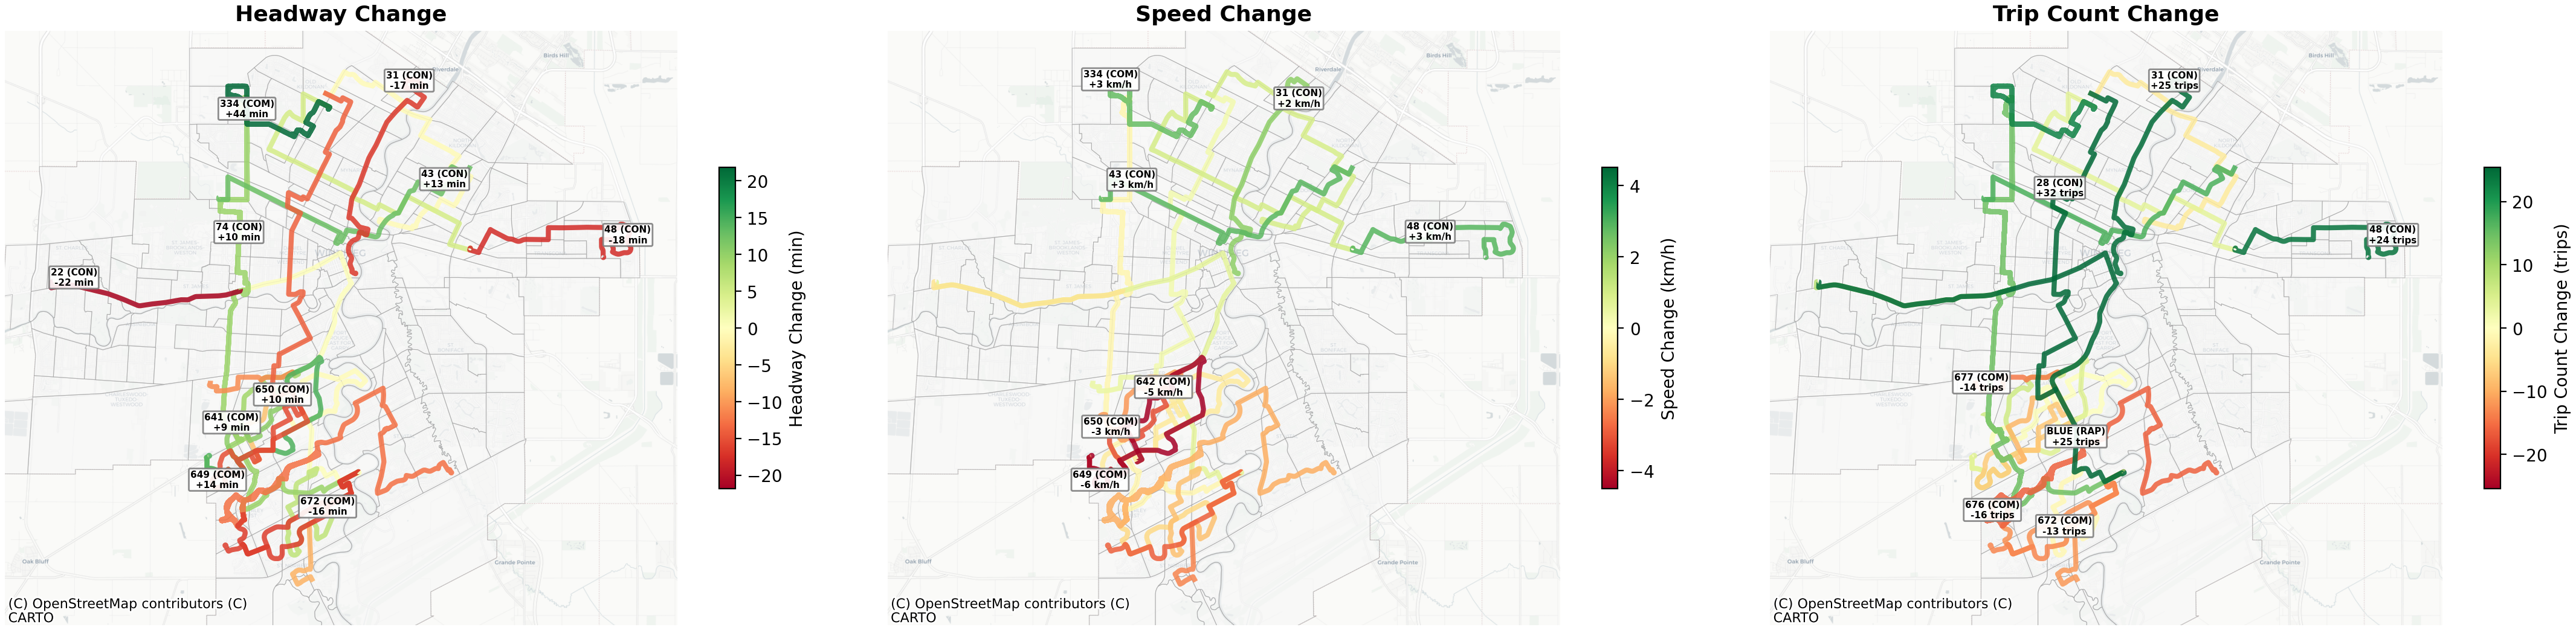
\includegraphics[width=0.9\textwidth]{prepost_combined}
\caption{Route-level pre/post maps: headway change (left), speed change (centre), trip count change (right). Green = improved, red = worsened.}
\label{fig:prepost}
\end{figure}

Figure~\ref{fig:prepost} maps these changes at the route level.
Mean headway remained flat (31.0 to 31.9~min), contradicting the premise
of frequency improvement. The network lost 1{,}265 stops ($-25\%$), 16 routes
($-18\%$), and 2{,}297 connections ($-33\%$). Table~\ref{tab:quintile}
shows the distributional impact by income quintile.

\begin{table}[H]
\centering\footnotesize
\caption{Distributional impact: transit accessibility by income quintile.
Q1 gained proximity from inner-city spine concentration while Q4/Q5 lost suburban coverage.}
\label{tab:quintile}
\begin{tabular}{lrrr}
\toprule
\textbf{Income Quintile} & \textbf{Pre-PTN} & \textbf{Current} & \textbf{Change} \\
\midrule
Q1 (lowest, inner-city) & 48.23 & 52.63 & $+9.1\%$ \\
Q2 & 37.79 & 38.28 & $+1.3\%$ \\
Q3 & 28.71 & 28.83 & $+0.4\%$ \\
Q4 & 25.58 & 20.63 & $-19.4\%$ \\
Q5 (highest, suburban) & 25.12 & 21.78 & $-13.3\%$ \\
\bottomrule
\end{tabular}
\end{table}

\subsection{Route Archetypes}

K-means clustering ($k=4$) reveals four distinct route archetypes
(Figure~\ref{fig:clustering}):
\begin{enumerate}
\item \textbf{High-frequency spine routes} (BLUE, FX2--4): $<$10~min headway, high boardings
\item \textbf{Medium-frequency corridors} (Frequent, Direct): 10--15~min headway
\item \textbf{Low-frequency feeders} (Connector): 15--30~min, transfer-dependent
\item \textbf{Minimal-service community} (Community, Limited Span): $>$30~min, evening gaps
\end{enumerate}

\begin{figure}[!htbp]
\centering
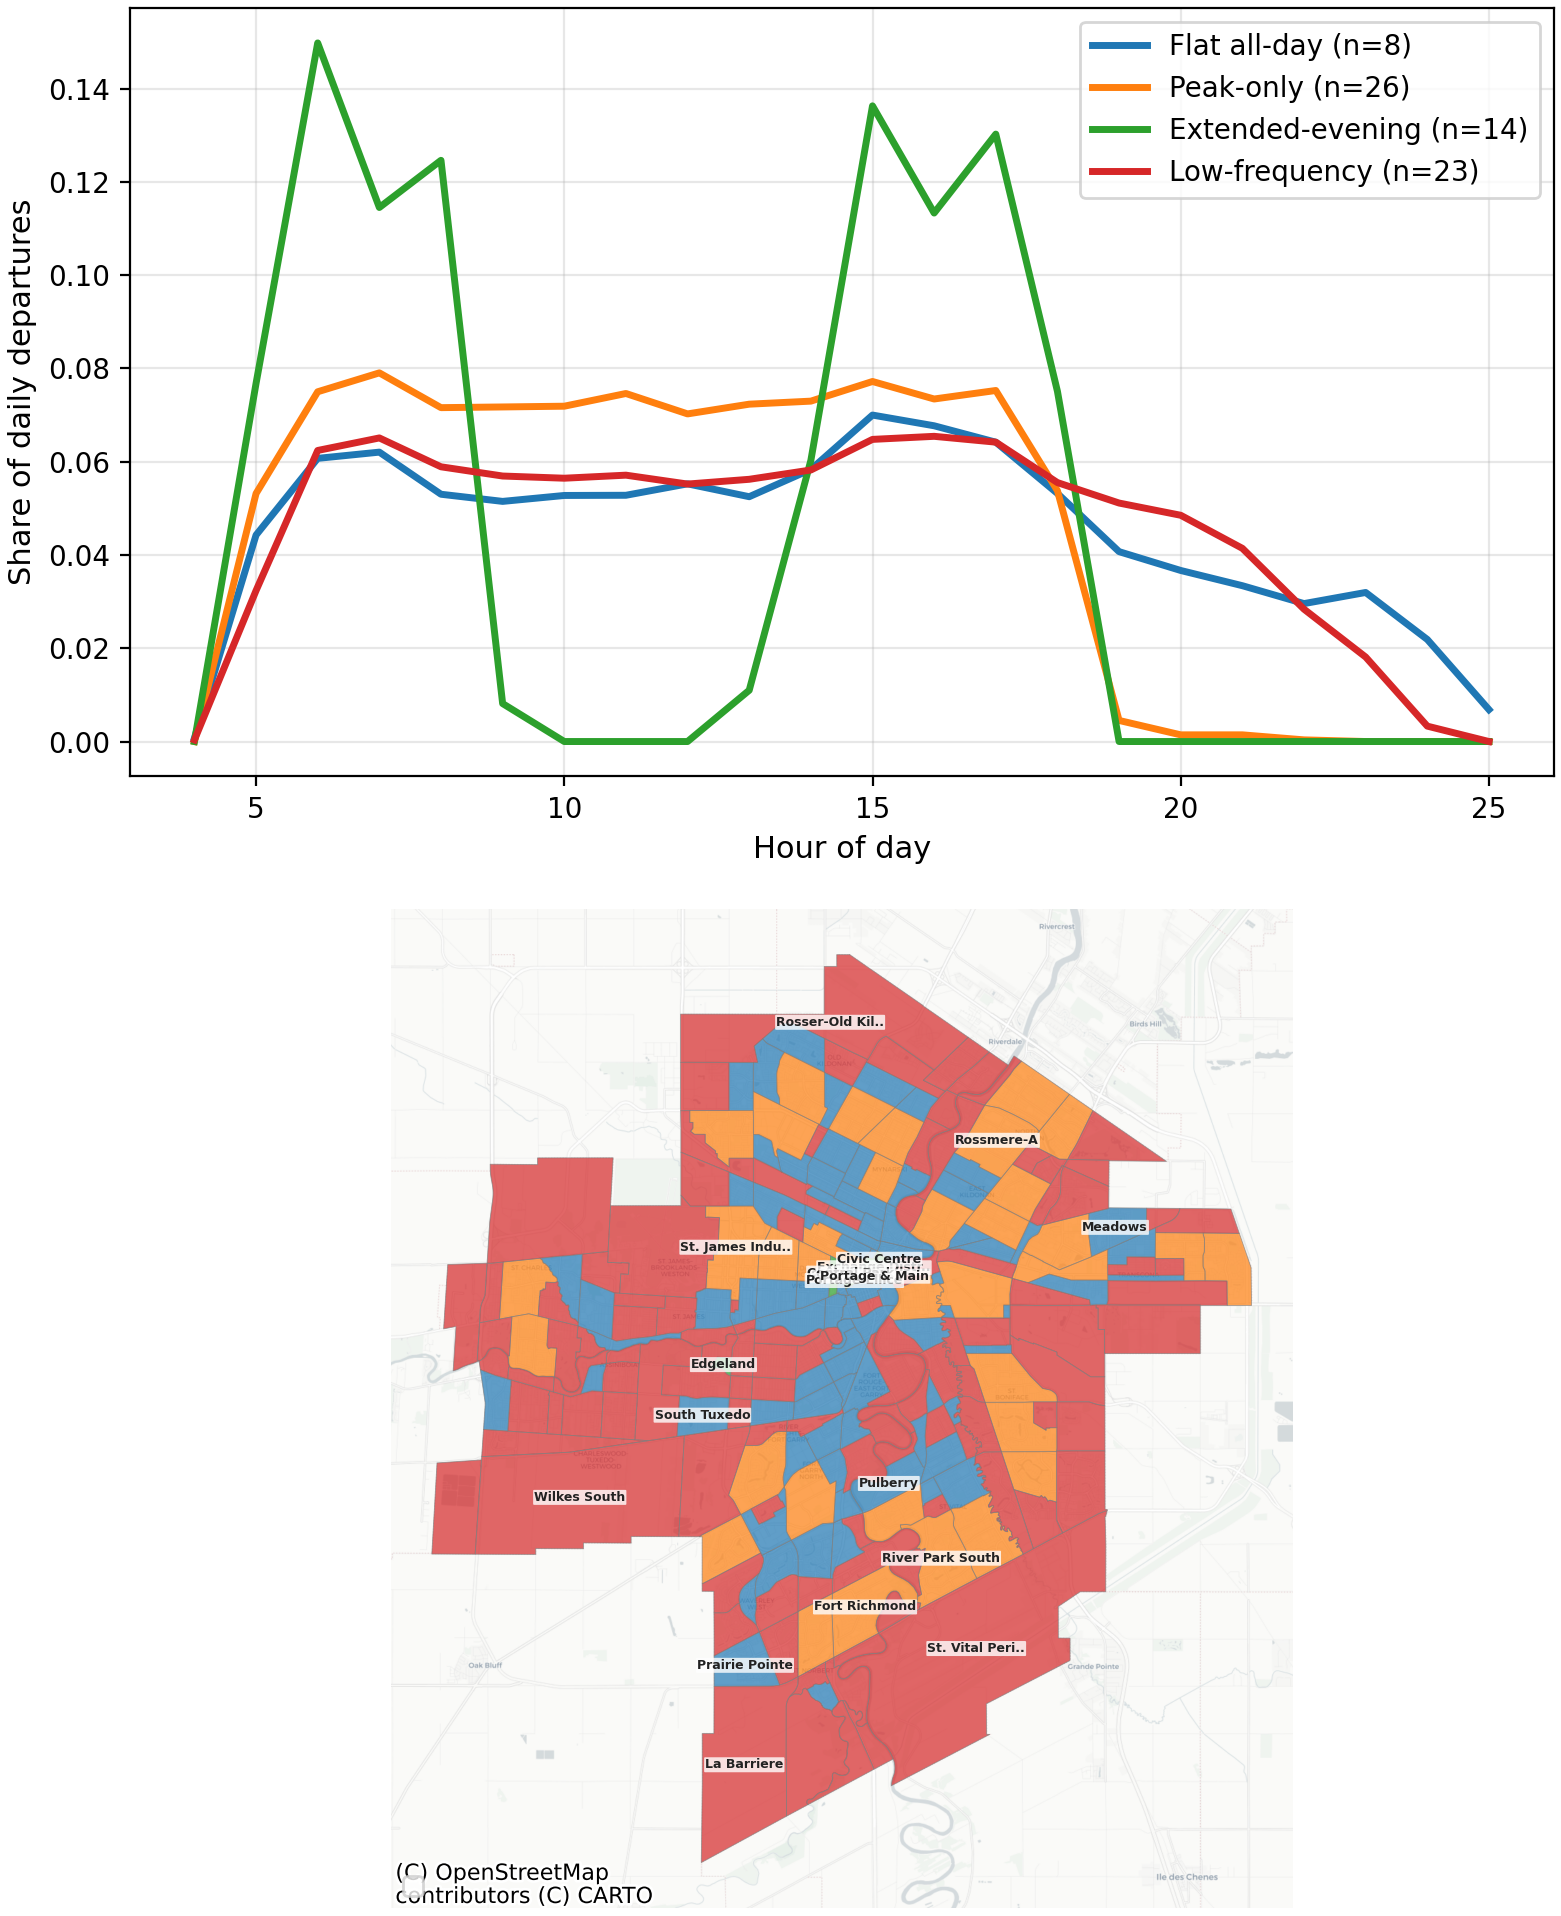
\includegraphics[width=0.85\textwidth]{clustering_combined}
\caption{Route clustering: hourly departure profiles for 4 archetypes (top) and neighbourhood service cluster map (bottom).
Silhouette score $s=0.40$ confirms moderate cluster separation.}
\label{fig:clustering}
\end{figure}

For neighbourhood service clusters, Ward hierarchical clustering validates the K-means assignment (Adjusted Rand Index $= 0.42$, moderate agreement). The Negative Binomial generalized linear model (GLM) identifies capacity-stressed routes predominantly in the Connector and Community tiers, where pass-up rates are highest.

\subsection{Classification Performance}

Random Forest achieves weighted F1=0.81 for coverage category prediction
(Figure~\ref{fig:classification}) using demographic features (population density, transit commute share, median household income, percentage of seniors 65+).
Naive Bayes achieves F1=0.71 and Gradient Boosting F1=0.80. The high predictive power of demographics alone confirms that coverage category is largely determined by \emph{who lives there}: neighbourhood income, transit commute share and population density are sufficient to predict service level without any schedule inputs. PCA on the 8 census features confirms the feature set: the first three components explain 77\% of variance (PC1 loads on transit and car commute, PC2 on cycling and seniors).

\begin{figure}[!htbp]
\centering
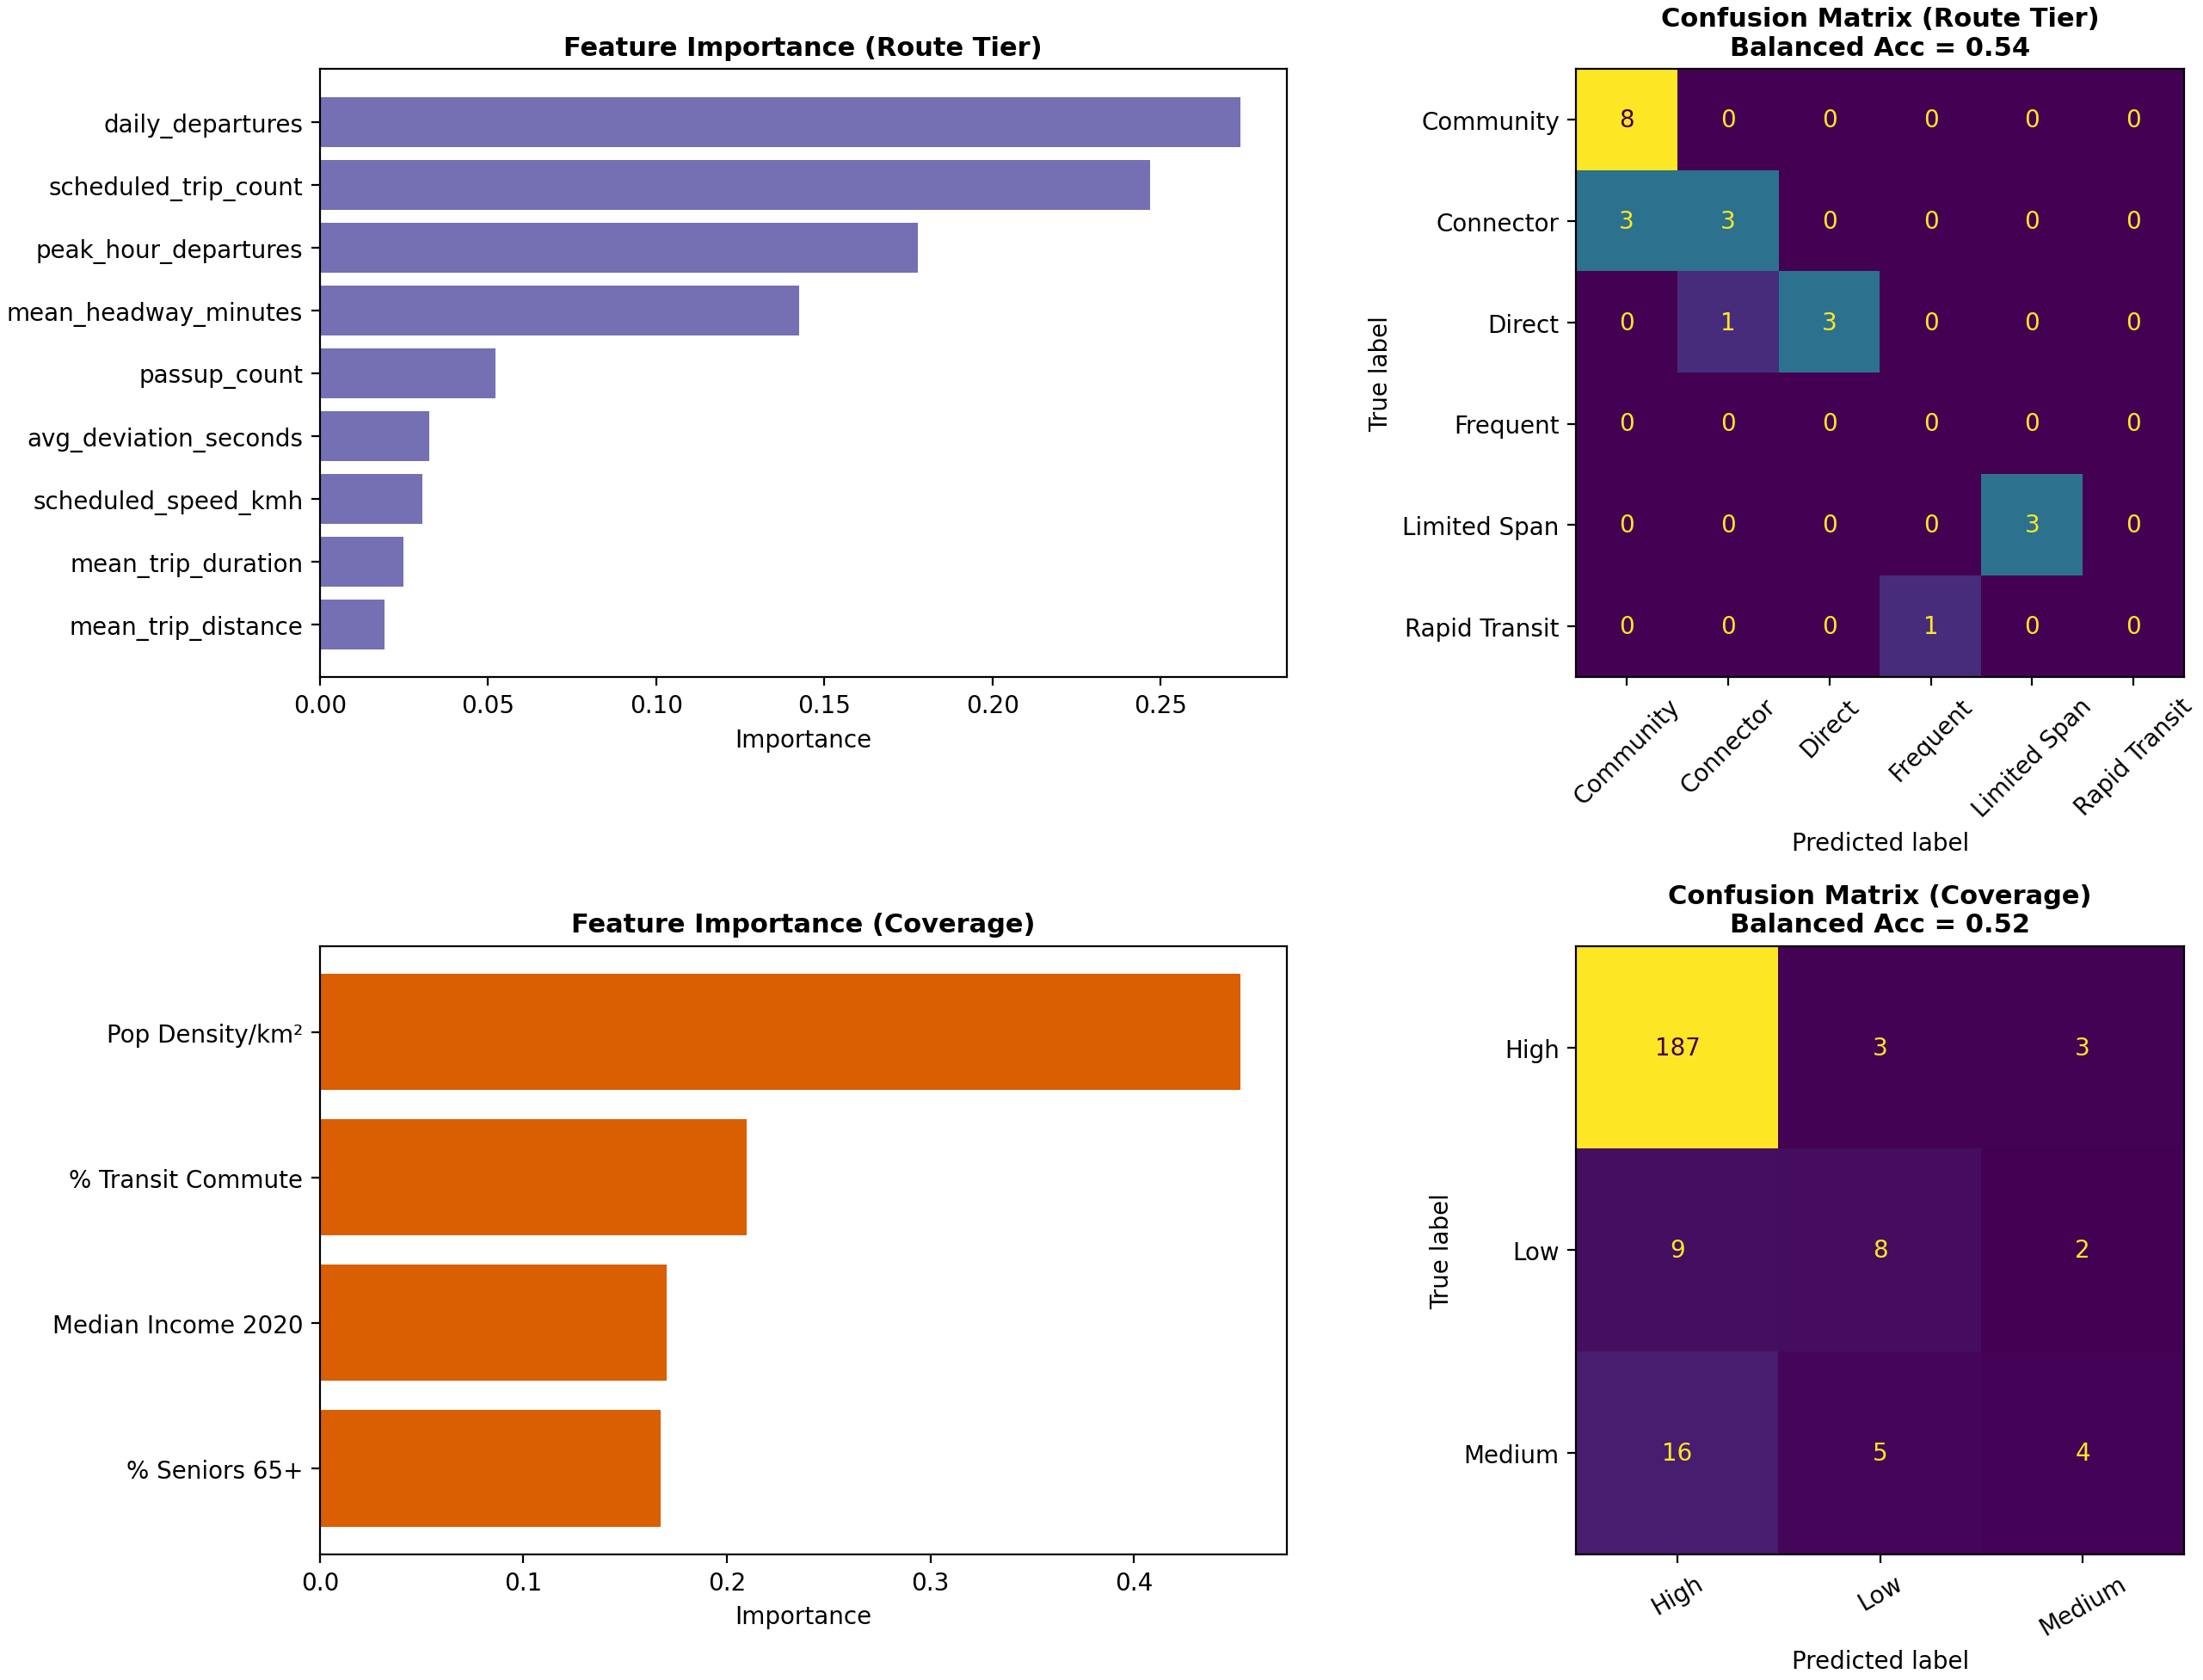
\includegraphics[width=0.85\textwidth]{classification_combined}
\caption{Classification results. Top row: route-tier classifier (schedule features). Bottom row: coverage classifier (demographic features). Population density and transit commute share are the top coverage predictors.}
\label{fig:classification}
\end{figure}

\subsection{Association Rules}

Apriori discovers 45 rules above $\text{lift} \geq 1.0$, of which 6 are
definitional (underserved $:=$ low\_income $\wedge$ low\_stop\_density).
The remaining 39 capture genuine co-occurrence patterns
(Figure~\ref{fig:rules_network}). Key patterns:
\begin{itemize}
\item $\{\text{low\_income}\} \Rightarrow
      \{\text{high\_immigrants}, \text{high\_transit\_commute}\}$
      (lift=1.78, conf.=0.59, support=0.295): wherever you find
      poverty, you find immigrant communities and transit dependency
\item $\{\text{high\_density}, \text{low\_income}\} \Rightarrow
      \{\text{high\_transit\_commute}\}$
      (lift=1.77, conf.=0.72, support=0.228): dense low-income
      neighbourhoods are transit-dependent by necessity, not choice
\end{itemize}
These patterns confirm that vulnerability indicators systematically co-occur with transit reliance, validating the BIZ survey finding that disabled (77\%), seniors (74\%) and low-income (70\%) riders are disproportionately dissatisfied.

\begin{figure}[!htbp]
\centering
\IfFileExists{figures/association_rules_network.png}{%
  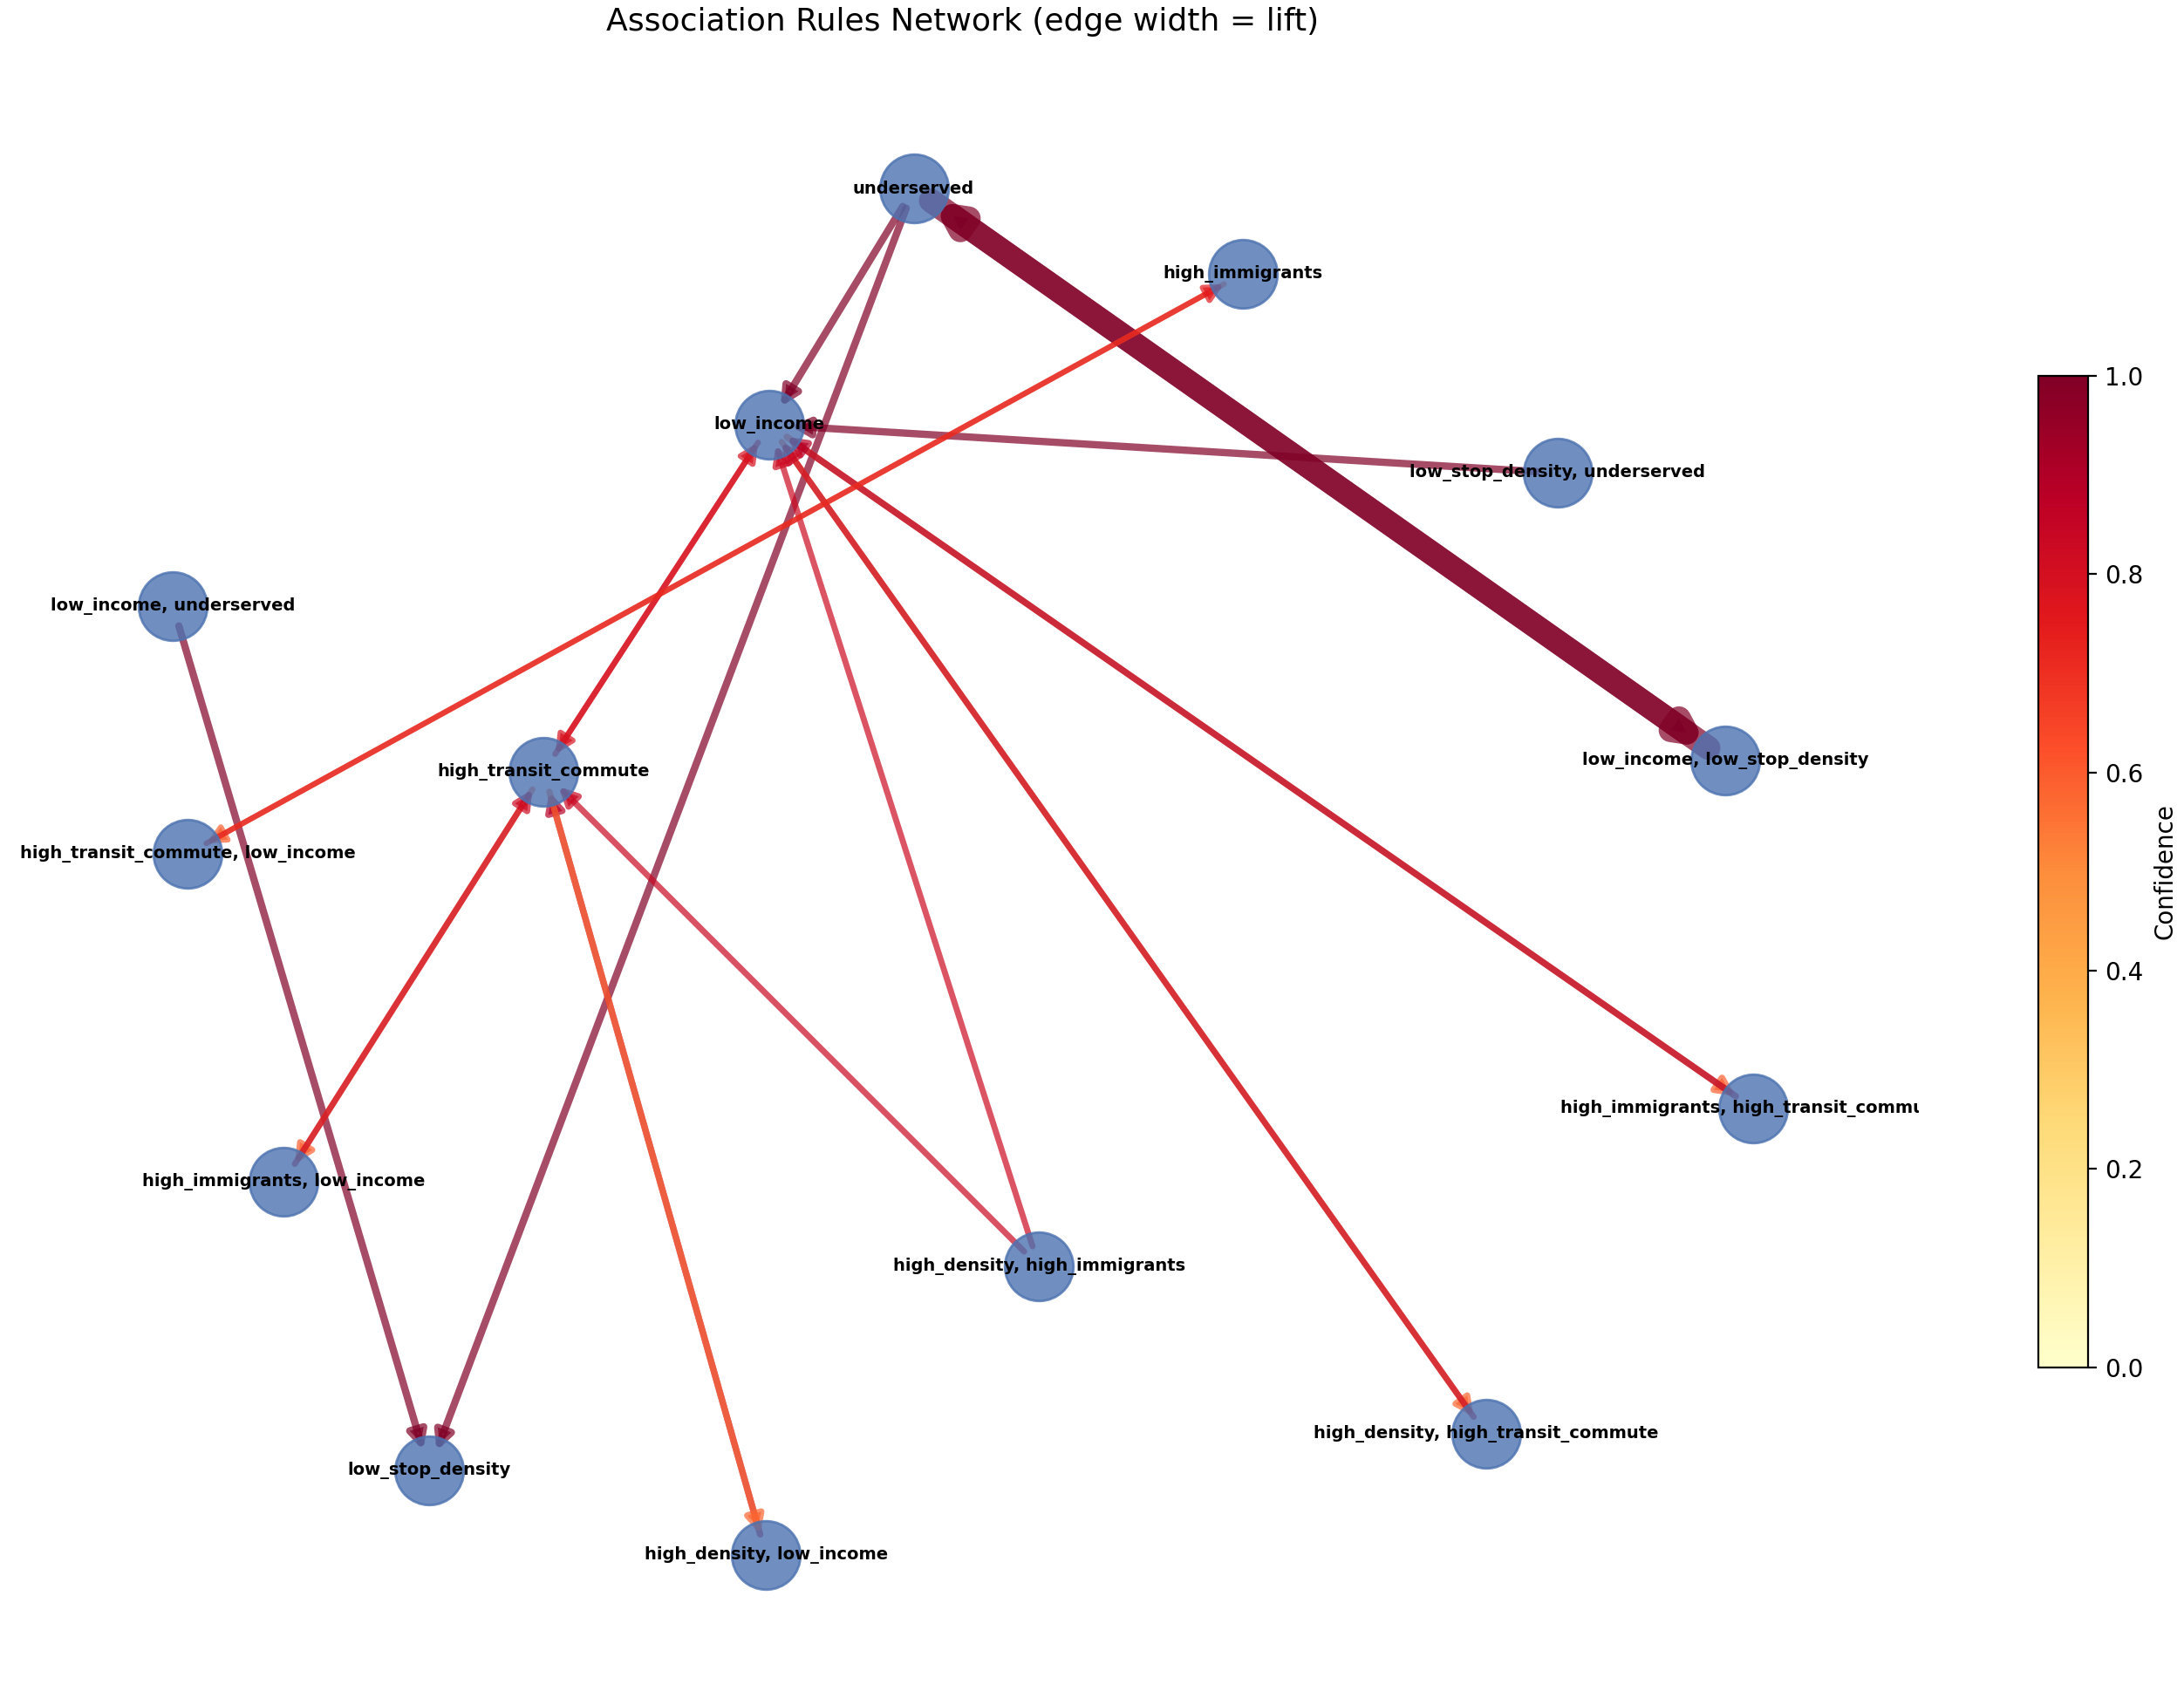
\includegraphics[width=0.75\textwidth]{figures/association_rules_network}%
}{%
  \fbox{\parbox{0.8\textwidth}{\centering\vspace{2em}\textbf{[FIGURE: Association Rules Network]}\vspace{2em}}}%
}
\caption{Association rules network: features as nodes, rules as directed edges
(width proportional to lift).}
\label{fig:rules_network}
\end{figure}

%=== CATHY WRITES: Network Communities ===
% TARGET: ~0.5 page. YOUR DATA: Run notebook 1.2
% KEY FRAMING: "Blind mathematical validation";Louvain knew nothing about
%   rail tracks; it rediscovered the CN/CP divide from graph topology alone
%   (Goods Movement Study 2022 confirms this physically)
% REPORT: N communities, alignment with rail corridors, top hubs by betweenness
% FIGURES: network_communities_pr2.png, community_boundary_alignment.png
\subsection{Network Communities}

Louvain community detection identifies 58 communities in the current network (3{,}873 nodes, 4{,}663 edges, clustering coefficient 0.013, assortativity 0.150, Figure~\ref{fig:communities}). Communities align with physical barriers: the CN and CP rail corridors create a ``rail divide'' that fragments the transit network into disconnected zones. The 240~km of rail, 793-acre CN Symington Yard and 230 at-grade crossings create natural community boundaries that the PTN grid design does not bridge. PageRank centrality identifies Unicity West Access (Polo Park area) as the most structurally important hub, consistent with the betweenness analysis.

%% CATHY: Expand this section (~250 words). Explain the ``blind mathematical
%% validation'' concept: Louvain found the CN/CP divide from graph topology alone,
%% with no geographic input. Discuss top hubs by betweenness centrality.
%% Stats: 58 communities, 3{,}873 nodes, 4{,}663 edges, clustering coefficient 0.013, assortativity 0.150.

\begin{figure}[!htbp]
\centering
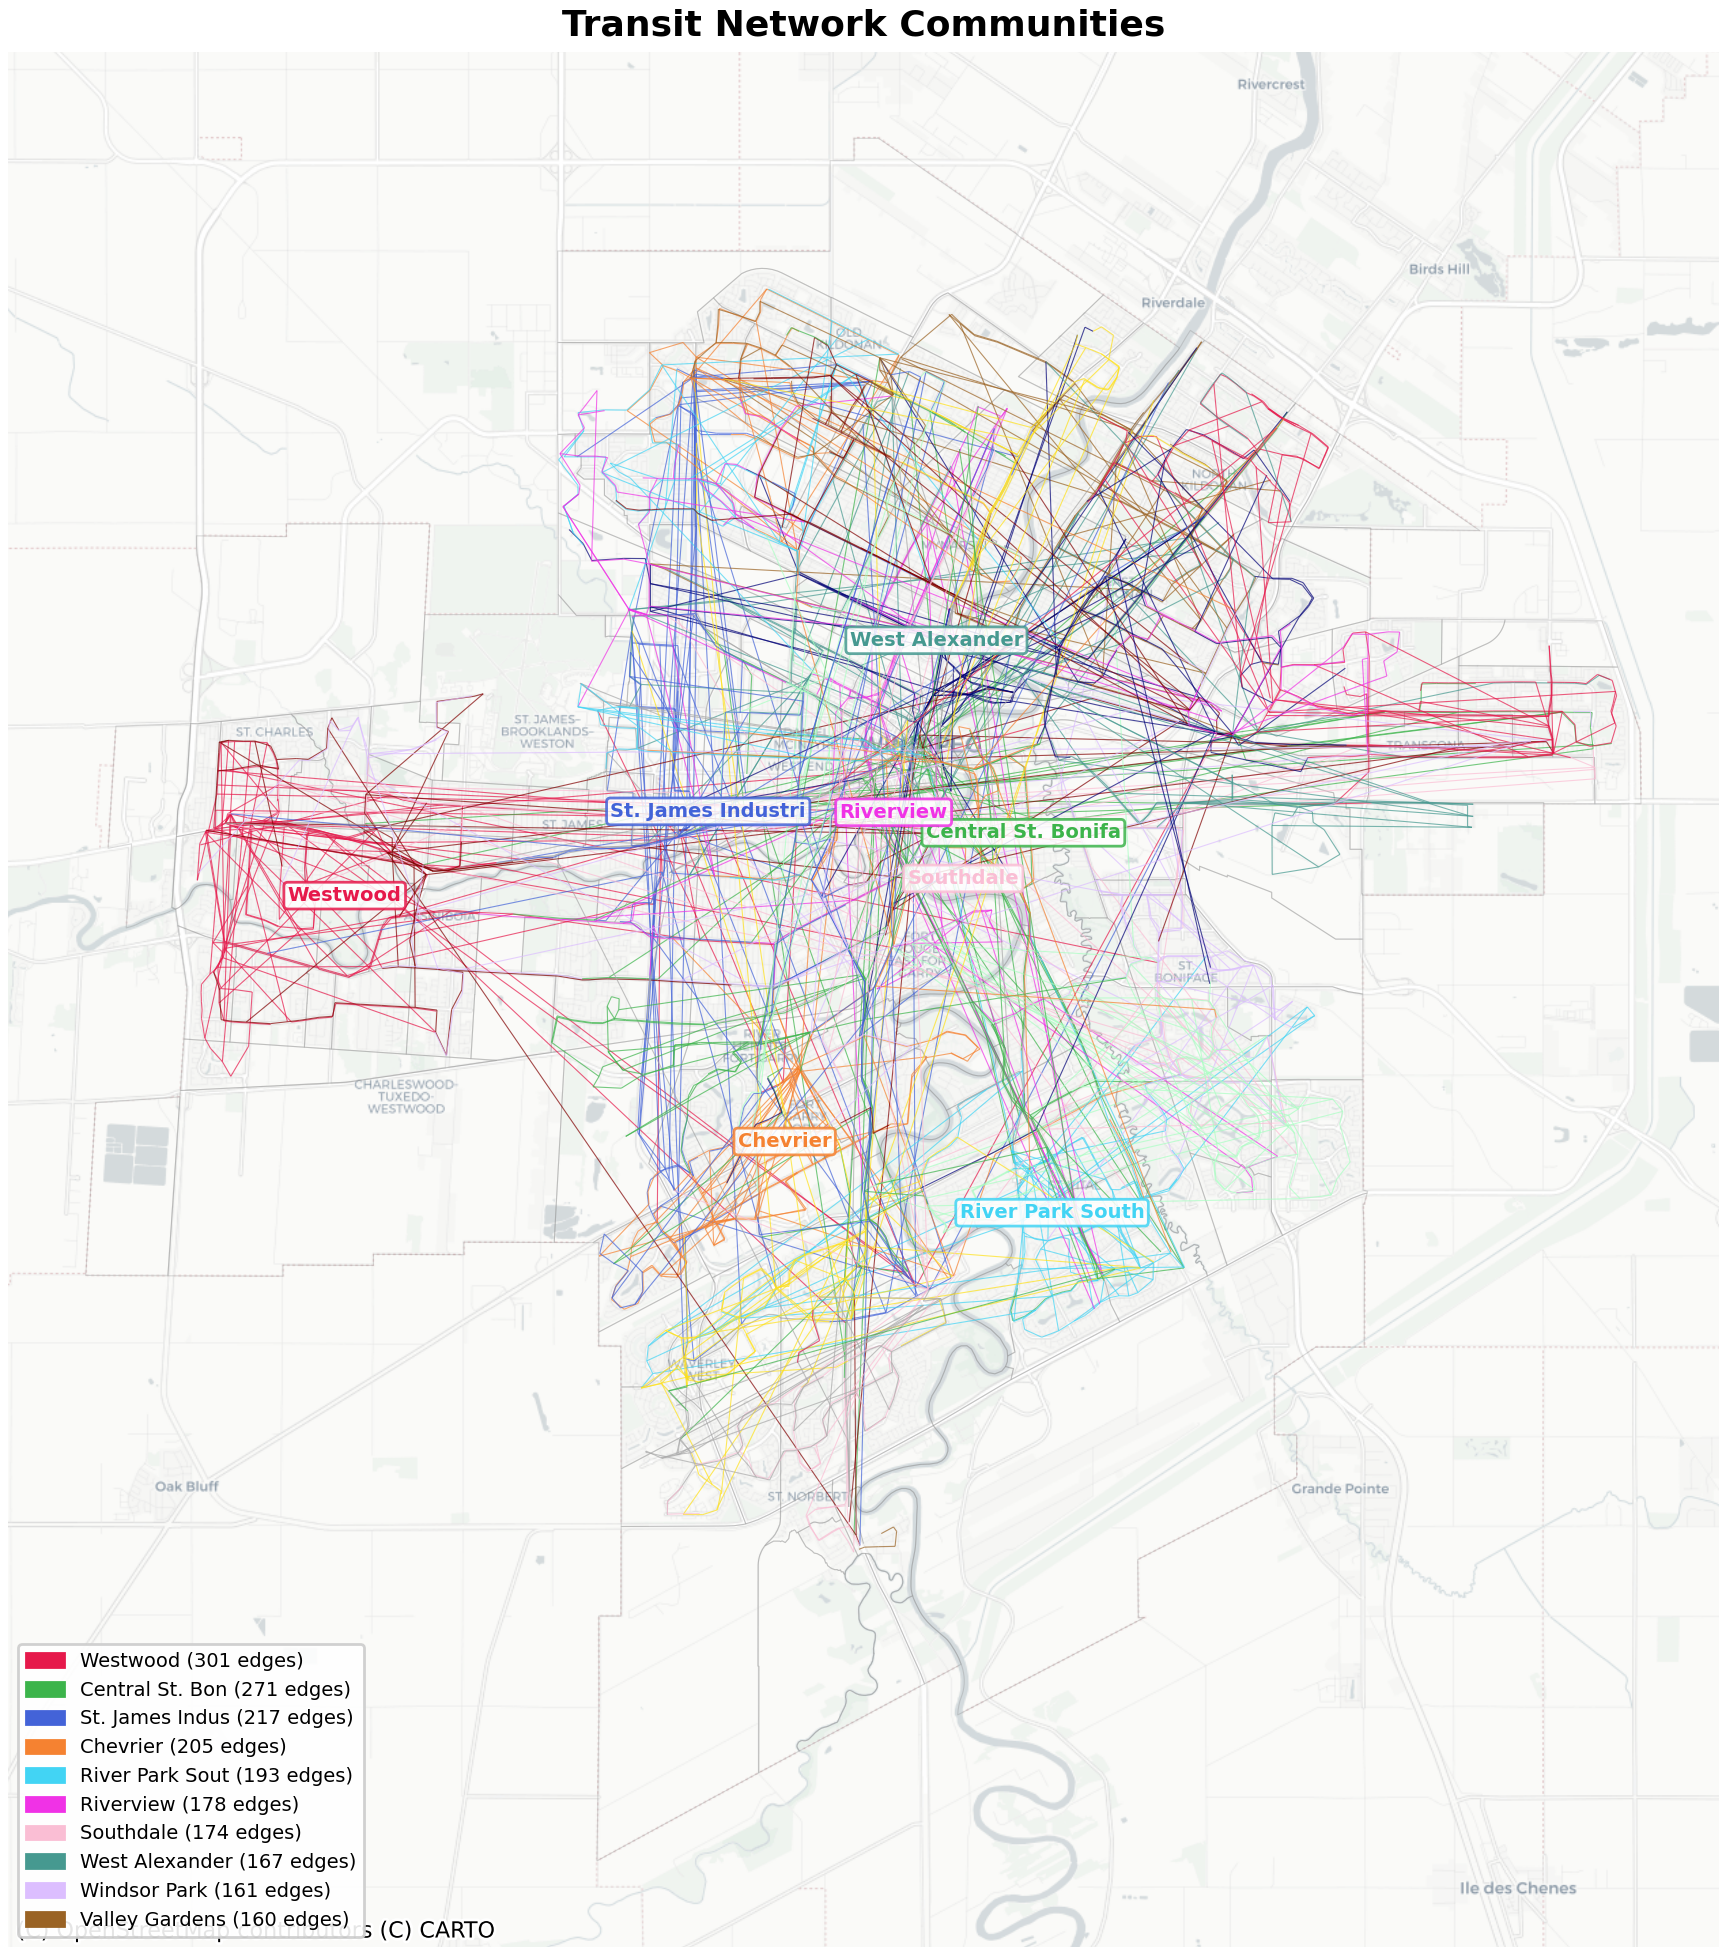
\includegraphics[width=0.75\textwidth,height=0.55\textheight,keepaspectratio]{network_communities_pr2}
\caption{Louvain network communities overlaid on neighbourhood boundaries.
Communities align with rail corridors, confirming the ``rail divide'' hypothesis.}
\label{fig:communities}
\end{figure}

%=== SUDIPTA WRITES: Equity by Income Quintile ===
% TARGET: ~0.5 page. VALUES: See docs/CLAIMS_SHEET.md
% REPLACE: All [NB~0.7] with real numbers
% KEY FRAMING: Lucas (2012) "Double Penalty";Q1 faces BOTH reduced transit access
%   (Penalty 1) AND fewer destinations (Penalty 2). PTN exacerbates by forcing transfers.
% FIGURE: equity_quintile.png
\subsection{Equity by Income Quintile}

We group Winnipeg's 237 neighbourhoods into five equal-sized income bands
(quintiles): Q1 is the lowest-income 20\% (median income \textasciitilde\$30K)
and Q5 is the highest-income 20\% (median income \textasciitilde\$54K).

Transit accessibility scores (Figure~\ref{fig:equity_quintile}) reveal an inverse income pattern: Q1 neighbourhoods have the \emph{highest} median access score (52.63), while Q5 has the lowest (21.78). The pattern is broadly inverse: Q1 (52.63) $>$ Q2 (38.28) $>$ Q3 (28.83), though Q4 (20.63) dips below Q5 (21.78), reflecting suburban pockets with marginally better feeder coverage. This reflects Winnipeg's urban geography: the poorest neighbourhoods are inner-city (Lord Selkirk Park, Spence, West End) with high stop density, while the wealthiest (Tuxedo, Wellington Crescent) are low-density suburbs far from transit spines. The equity concern is not proximity but \emph{service quality}: inner-city residents face higher transfer friction, longer wait times and pass-up denials despite living near more stops.

%% SUDIPTA: Expand this section (~250 words). Discuss Lucas (2012)
%% ``Double Penalty'': Q1 has proximity but faces service quality barriers.
%% Key values: Q1=52.63, Q2=38.28, Q3=28.83, Q4=20.63, Q5=21.78.

\begin{figure}[!htbp]
\centering
\IfFileExists{figures/equity_quintile.png}{%
  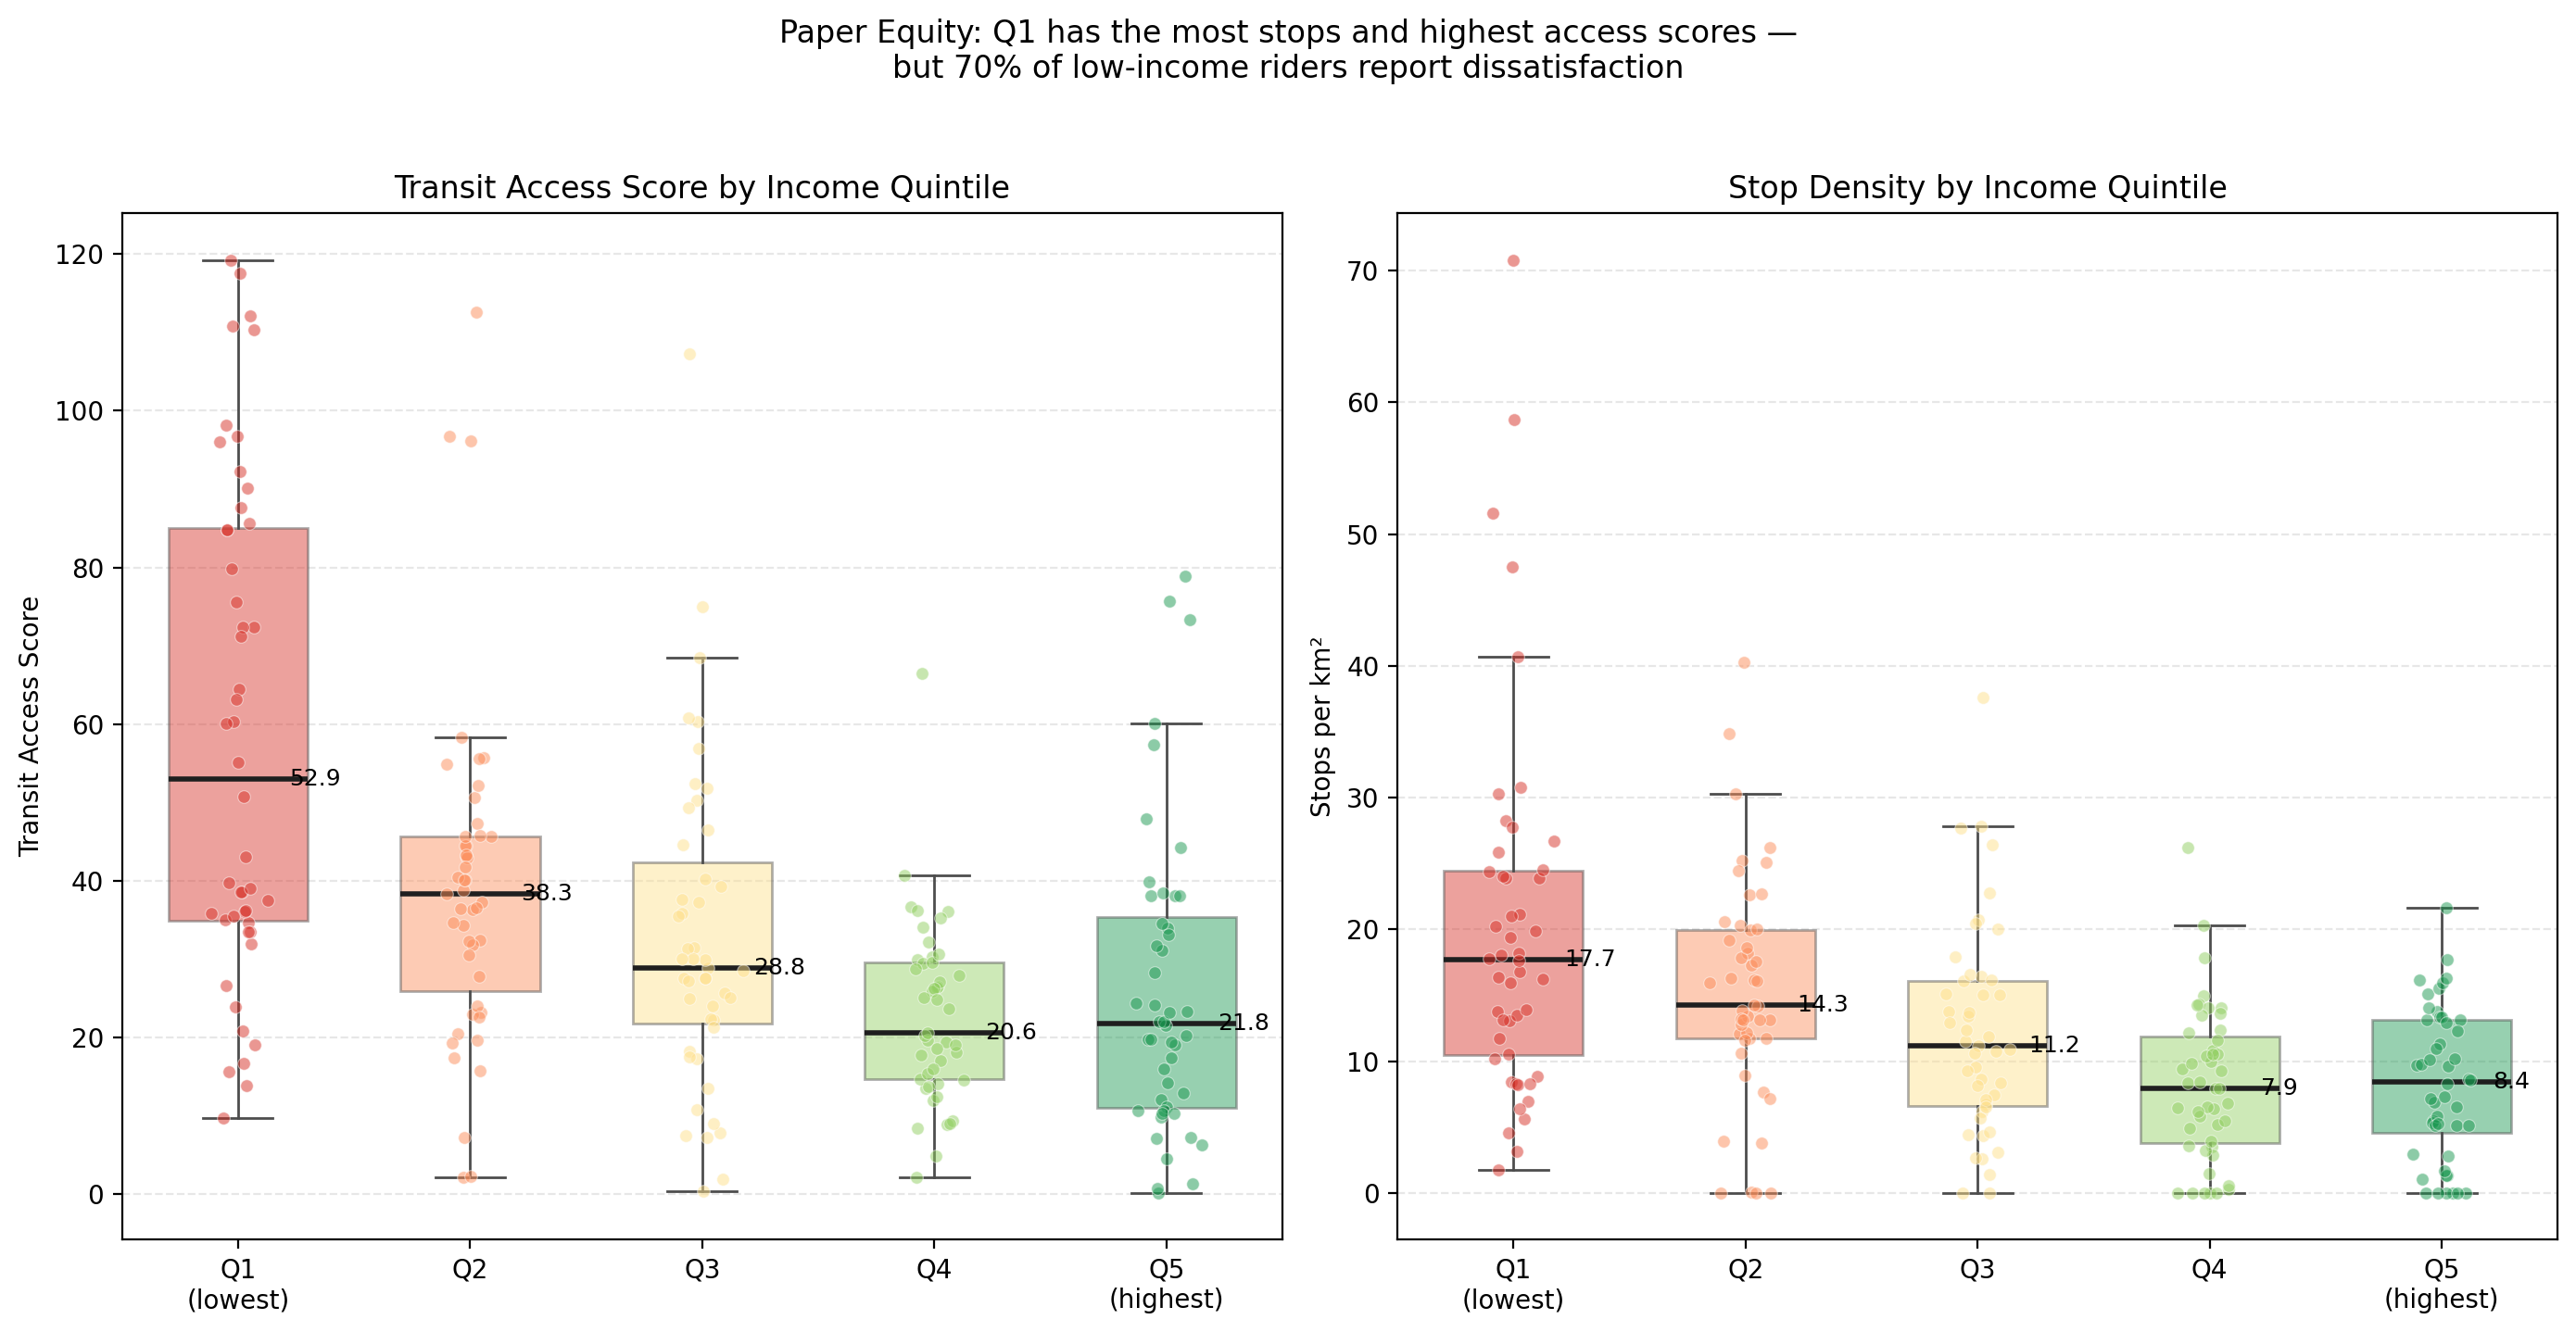
\includegraphics[width=0.85\textwidth]{figures/equity_quintile}%
}{%
  \fbox{\parbox{0.8\textwidth}{\centering\vspace{2em}\textbf{[FIGURE: Equity by Income Quintile]}\vspace{2em}}}%
}
\caption{Box plots of transit access score (left) and stop density (right) by income quintile. Q1 (lowest income, inner-city) has the highest median access and widest spread. The subtitle captures the paradox: proximity does not equal service quality.}
\label{fig:equity_quintile}
\end{figure}

% =========================================================
%% INSTRUCTIONS FOR SUDIPTA:
%% TARGET: ~0.75 pages (approx. 350 words).
%% 1. This section merges your MISSING PR2 coverage maps with your final poverty analysis.
%% 2. Discuss the coverage change map (fig:coverage_change). Where did stop density drop most?
%% 3. Discuss the underserved neighbourhood ranking (fig:underserved_ranks). Who lost out?
%% 4. Link this to poverty: The counterfactual model reprioritized 209 out of 237 neighbourhoods (88.2%).
%% 5. Highlight the top 3 gainers: Alpine Place (+44 ranks), Valhalla (+37), Pembina Strip (+36).
% =========================================================
\subsection{Poverty Overlay and Coverage Densification}

Poverty overlay analysis examines whether LIM-AT poverty zones have systematically worse transit access. Figure~\ref{fig:poverty_correlation} plots income against access for all 237 neighbourhoods, revealing that lower-income areas cluster at \emph{higher} access scores, the inverse of what standard equity models predict. Figure~\ref{fig:coverage_change} maps the stop-density changes, and Figure~\ref{fig:underserved_ranks} ranks the most underserved neighbourhoods.

%% SUDIPTA: Expand this section (~250 words). Describe the income-access
%% correlation pattern visible in Figure~\ref{fig:poverty_correlation}.
%% Key values: 209/237 (88.2\%) neighbourhoods reprioritized under equity weighting.
%% Top gainers: Alpine Place (+44 ranks), Valhalla (+37), Pembina Strip (+36).
%% Cite: Lucas (2012) ``Double Penalty'', Allen \& Farber (2020).

\begin{figure}[!htbp]
\centering
\IfFileExists{figures/poverty_correlation.png}{%
  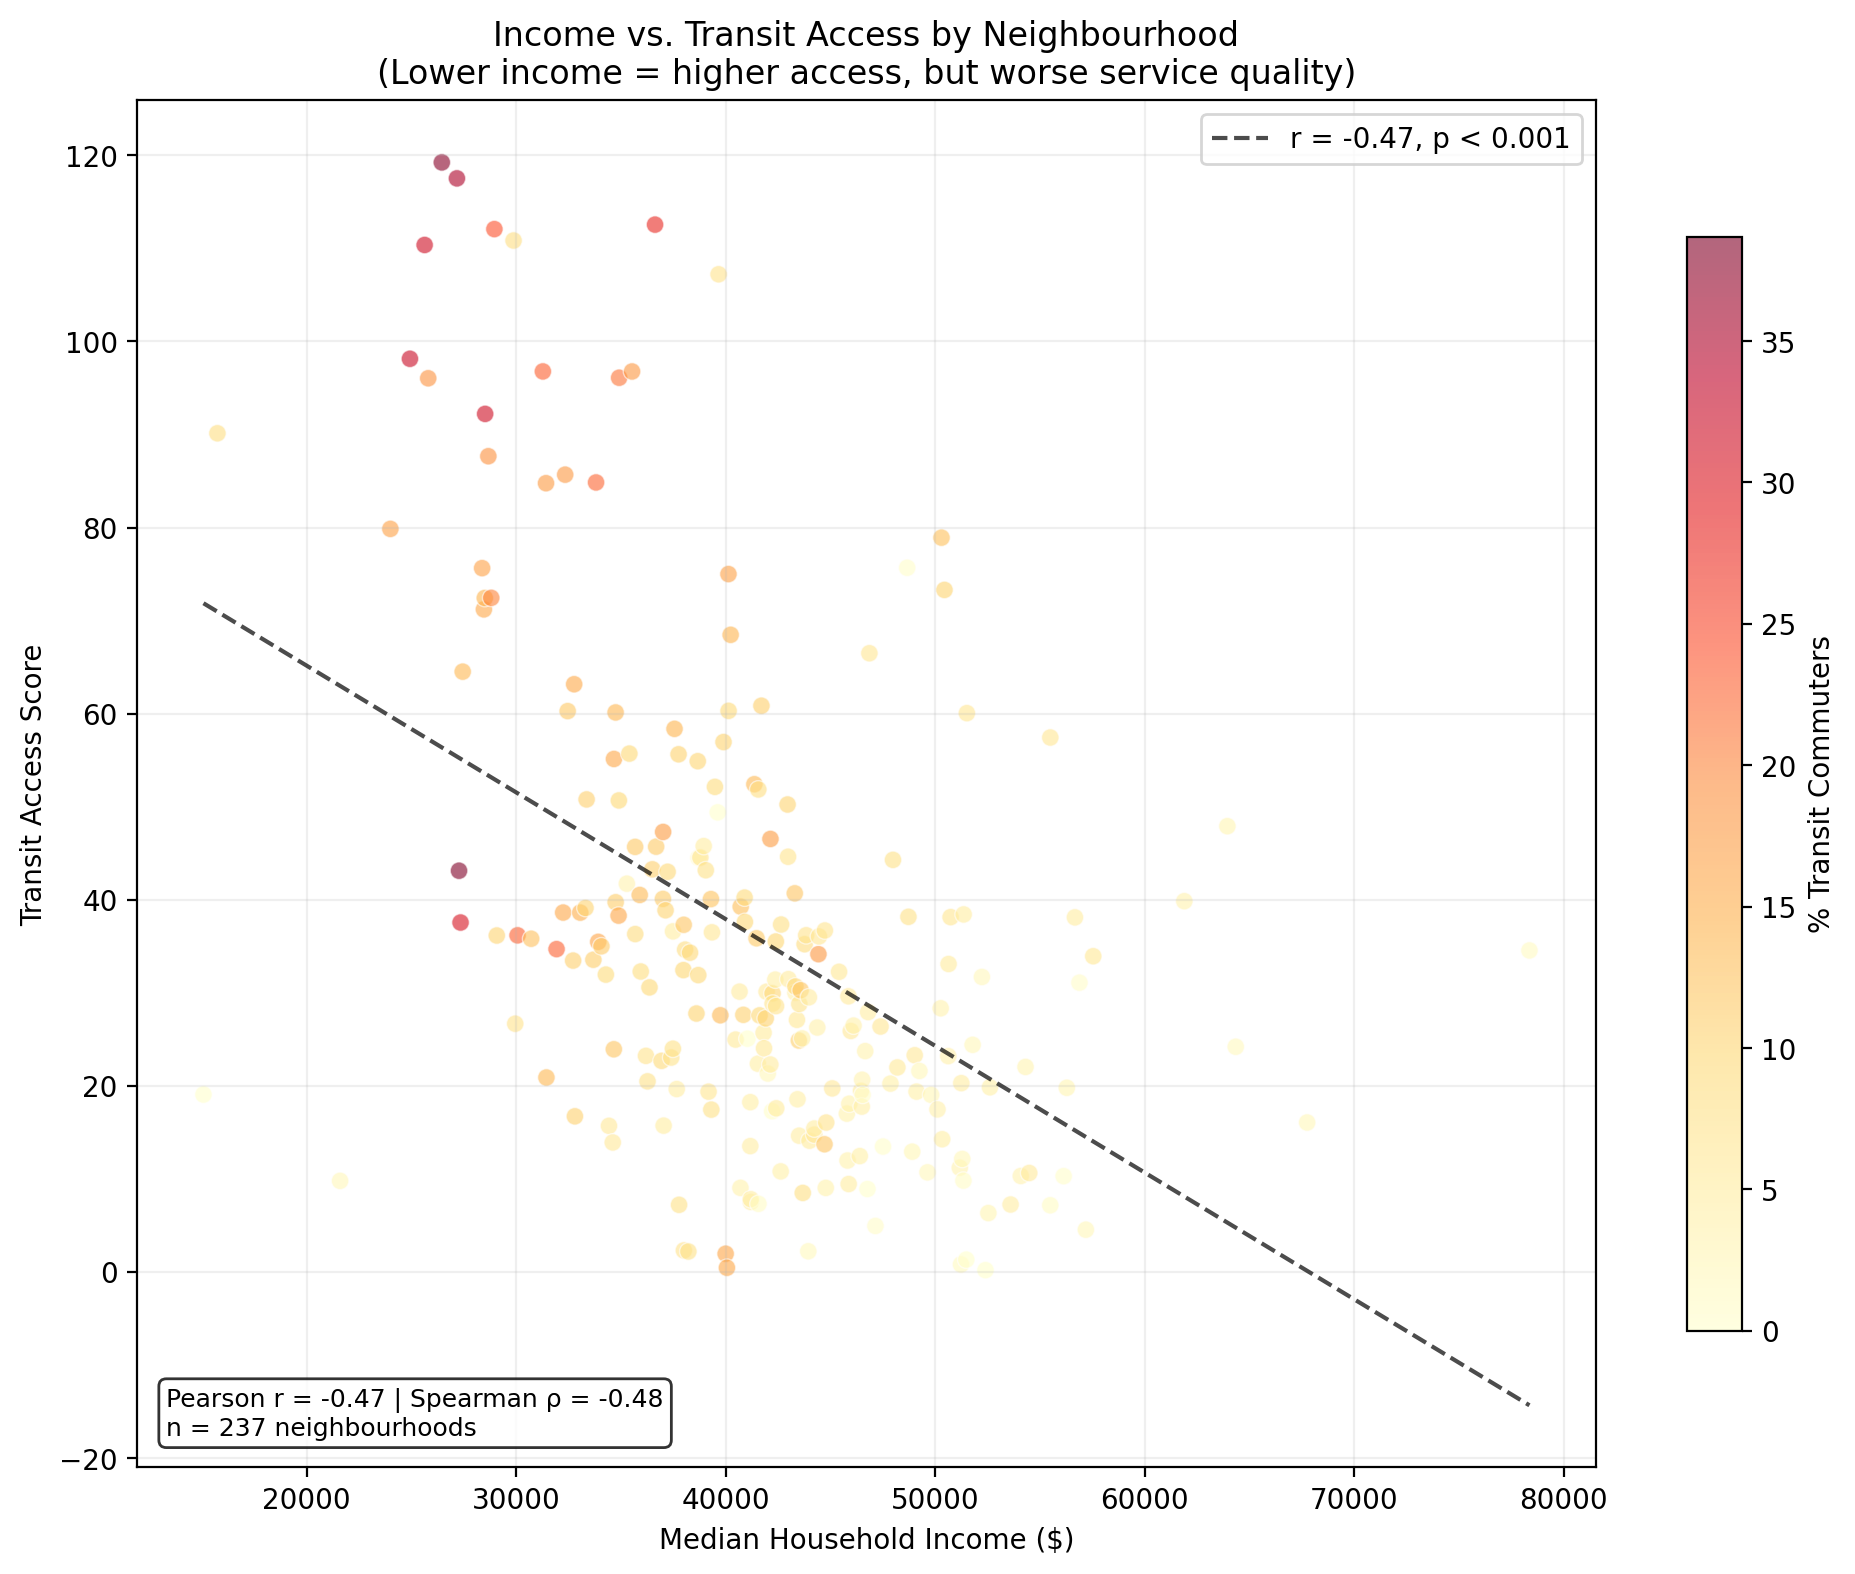
\includegraphics[width=0.85\textwidth]{figures/poverty_correlation}%
}{%
  \fbox{\parbox{0.8\textwidth}{\centering\vspace{2em}\textbf{[FIGURE: Poverty-Transit Correlation]}\vspace{2em}}}%
}
\caption{Income vs.\ transit access by neighbourhood ($r = -0.47$, dashed regression line). Colour encodes transit commute share. Lower income correlates with higher access scores, but not better service quality.}
\label{fig:poverty_correlation}
\end{figure}

\begin{figure}[!htbp]
\centering
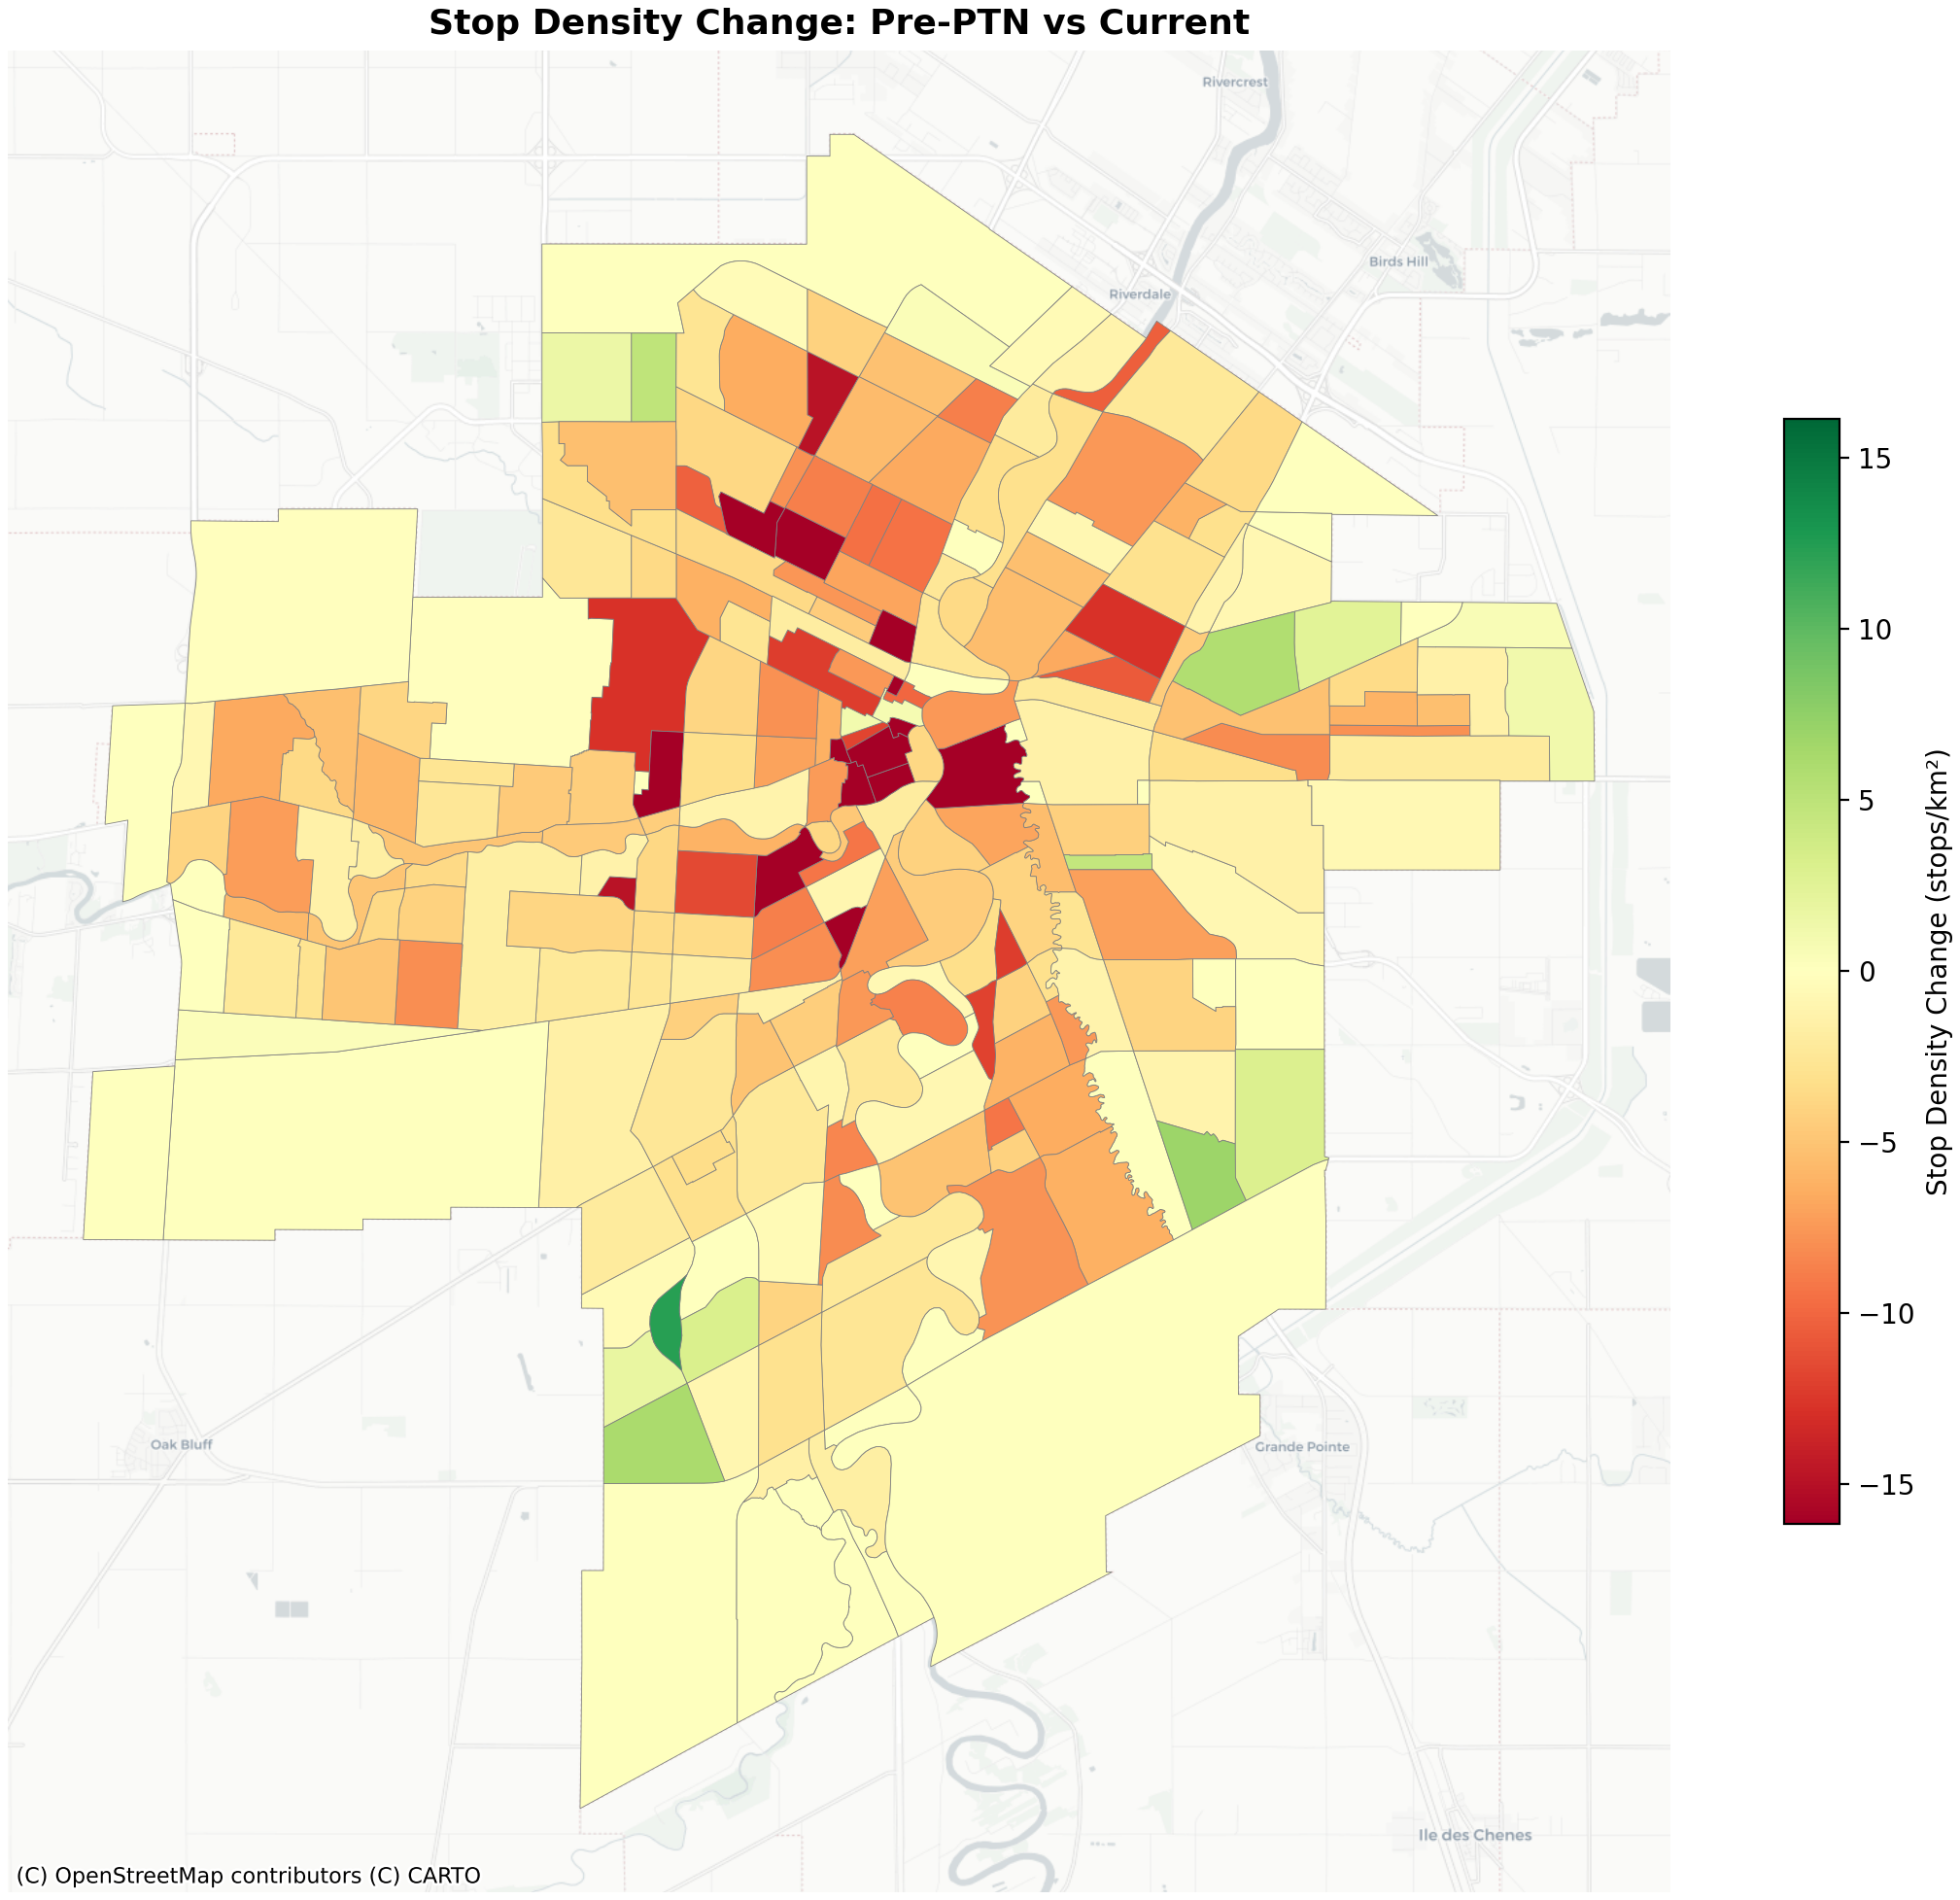
\includegraphics[width=0.8\textwidth]{coverage_change_map}
\caption{Coverage change choropleth comparing pre-PTN and current stop density.}
\label{fig:coverage_change}
\end{figure}

\begin{figure}[!htbp]
\centering
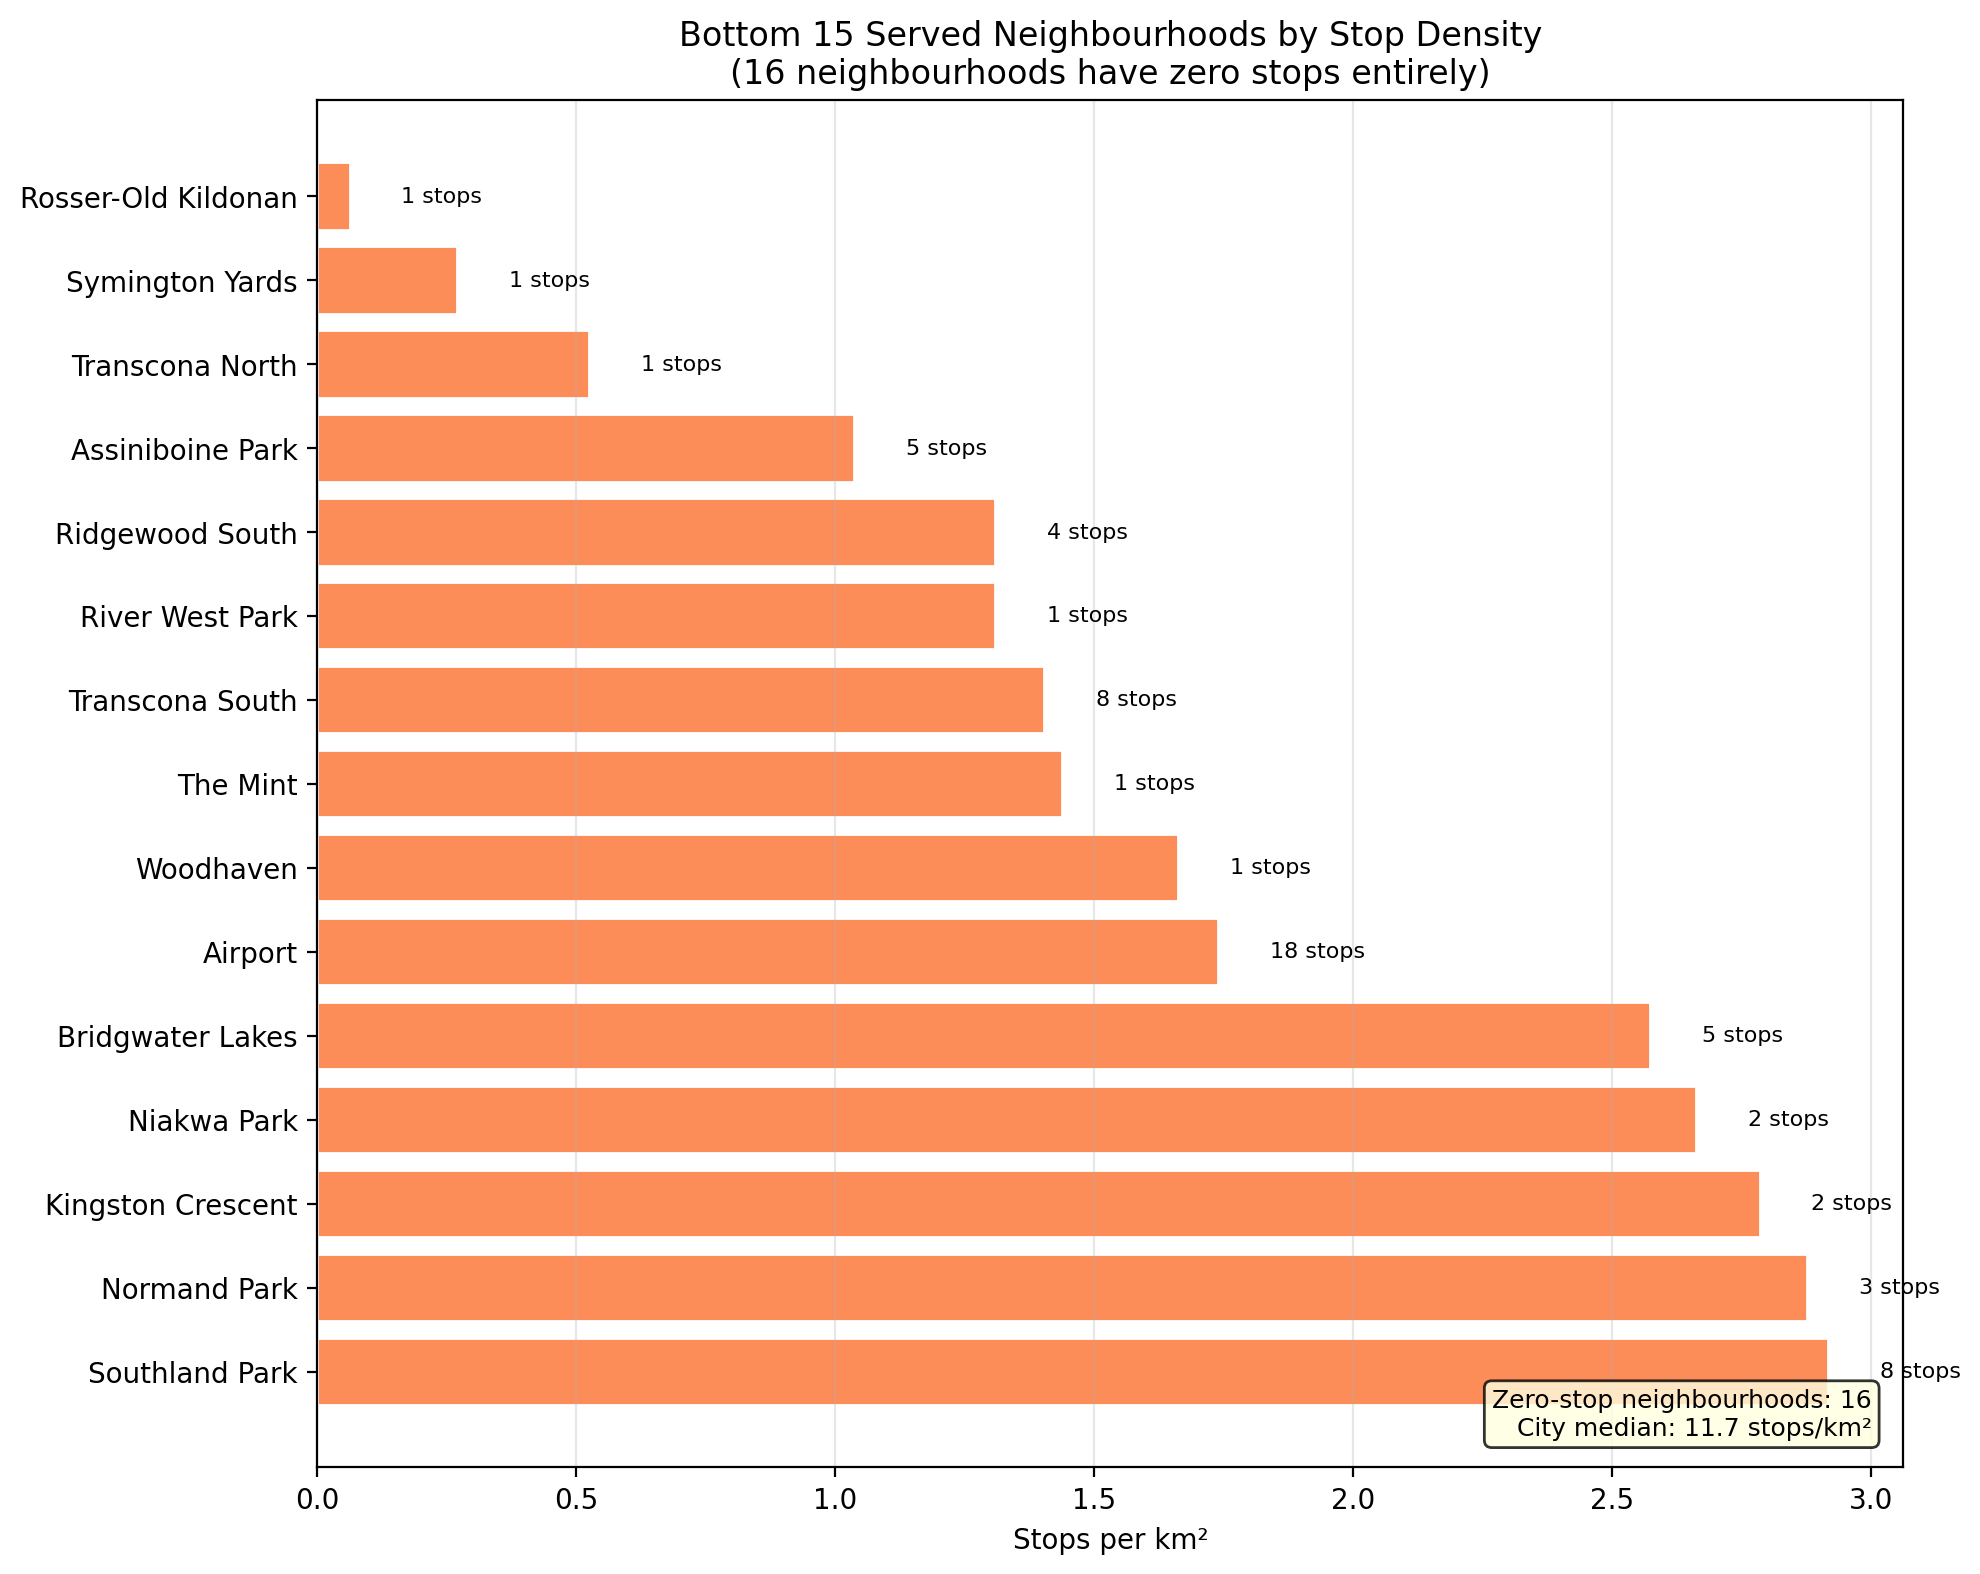
\includegraphics[width=0.8\textwidth]{underserved_neighbourhoods}
\caption{Bottom 15 underserved neighbourhoods by current stop density.}
\label{fig:underserved_ranks}
\end{figure}

\subsection{Prescriptive Counterfactual Results}

Our equity-weighted objective function reranks neighbourhoods
(Figure~\ref{fig:counterfactual}) by multiplying transit access scores with
vulnerability indices (z-scored income, transit dependency, seniors percentage).
This reprioritizes 88.2\% of neighbourhoods
(209 of 237): areas like Alpine Place (+44 ranks), Valhalla (+37) and
Pembina Strip (+36) move up, while affluent suburbs with low vulnerability
move down. This demonstrates that the \emph{same data} produces different
prioritization depending on the objective function. The choice of optimization
target is itself a policy decision with distributional consequences.

\begin{figure}[!htbp]
\centering
\IfFileExists{figures/counterfactual_rerank.png}{%
  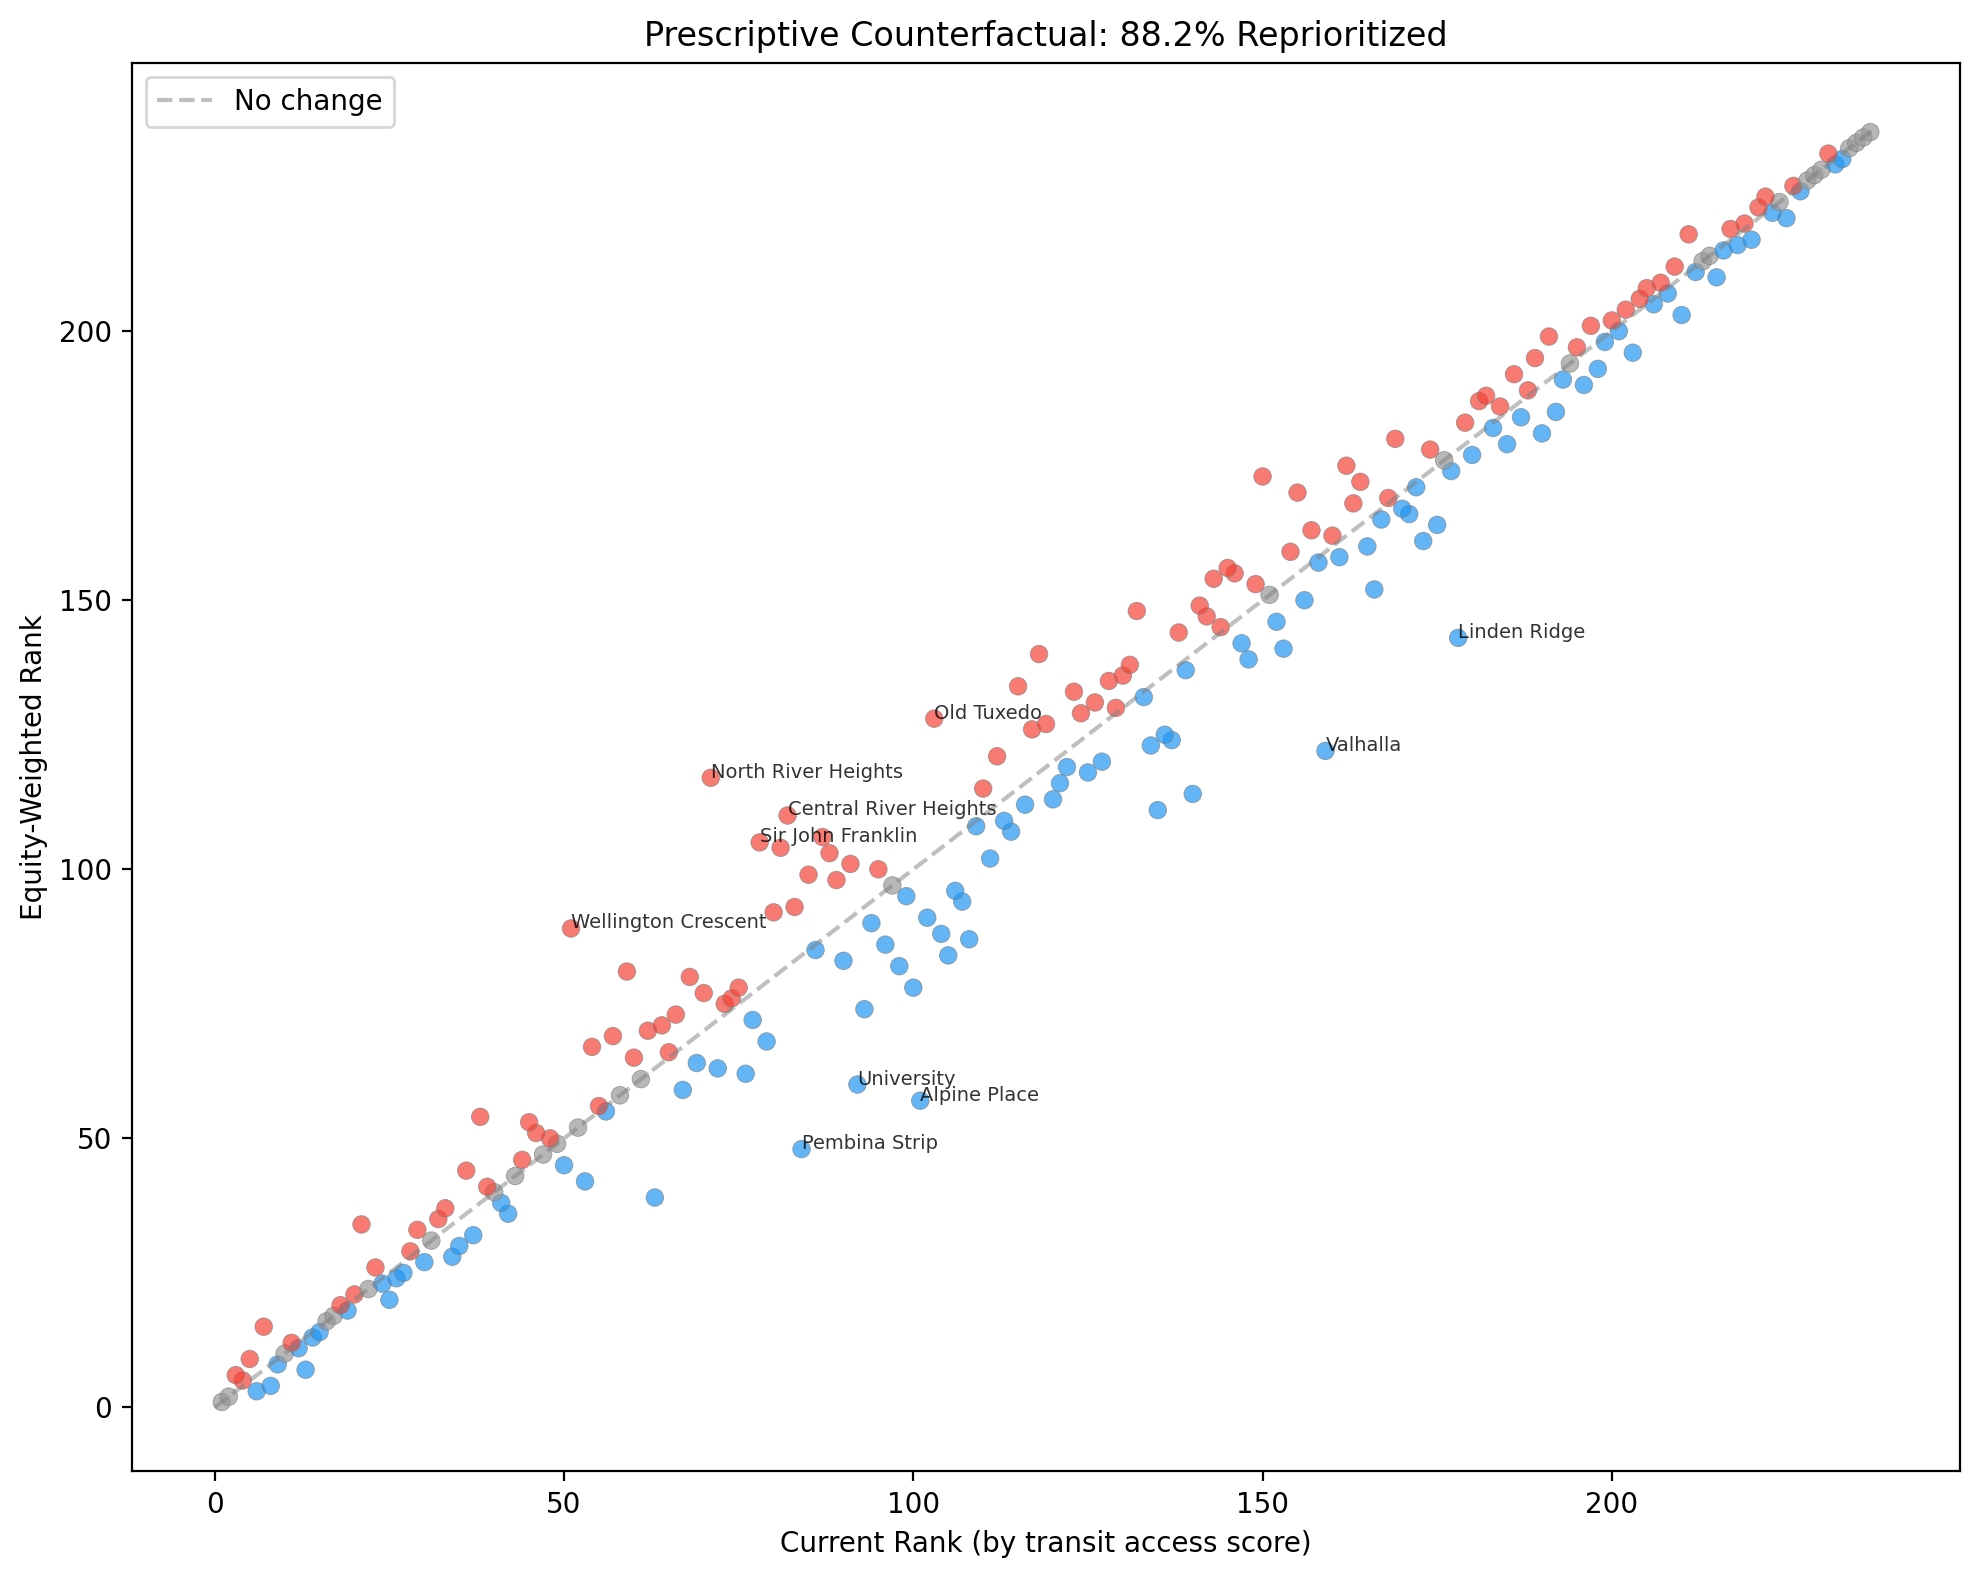
\includegraphics[width=0.85\textwidth]{figures/counterfactual_rerank}%
}{%
  \fbox{\parbox{0.8\textwidth}{\centering\vspace{2em}\textbf{[FIGURE: Prescriptive Counterfactual Reranking]}\vspace{2em}}}%
}
\caption{Prescriptive counterfactual: current rank vs.\ equity-weighted rank.
Points below the diagonal gained priority under equity weighting, while those above lost priority.}
\label{fig:counterfactual}
\end{figure}% =========================================================
\section{Discussion}
% =========================================================

\textbf{Paper equity vs.\ lived equity.} Our proximity model gives inner-city neighbourhoods like Lord Selkirk Park and Spence the highest transit scores in the city. The BIZ survey shows these same neighbourhoods report 70\% dissatisfaction. The model counts nearby stops. It cannot count the buses that pass you up, the transfers that don't connect, or the sidewalks buried under snow from November to March. Q1 neighbourhoods gained 9.1\% in proximity after the PTN launch, yet a separate rider survey found 70\% of low-income respondents dissatisfied. The PTN improved the score while degrading the experience. The association rules caught what the proximity model missed: \{underserved\} co-occurs with \{low\_income, low\_stop\_density\} not because these neighbourhoods lack nearby stops, but because the service at those stops has degraded. A rider taking the FX3 at 7:22 needs Route~74 at 7:53. Miss it by two minutes and the next one is at 8:11, 18 minutes in the cold. The 75-minute transfer window started at 7:22. By the time the second leg finishes, it may have expired. For a minimum-wage worker, that is a second fare they cannot afford.

\textbf{Design vs.\ operations.} Stantec built a geometry-first grid using proprietary origin-destination models, but publicly available Freedom of Information and Protection of Privacy Act (FIPPA) responses from late 2024 and early 2025, filed months before the PTN launch, show the City lacked the operational backend to run it. They have no formal policies for adjusting schedules (FIPPA~25-02-0253), no ability to track staff vacancies (25-02-0262), and no safety tracking (24-12-2017). The design might look optimal on a map, but it failed because it assumed perfect operational execution that Winnipeg Transit does not have.

\textbf{Limitations.} Census 2021 income data references 2020, a COVID year that may understate recovery incomes. The BIZ survey is self-selected ($n=1{,}395$) and likely overrepresents dissatisfied riders. The GPS data gap (Sep--Oct 2025) reduces on-time performance sample size.

\textbf{Edmonton comparison.}
Edmonton's April 2021 redesign achieved over 15\% ridership growth by 2024 through iterative post-launch adjustments, historically higher per-capita spending (CCPA 2018 documented \$335 vs.\ \$200 based on 2015 Canadian Urban Transit Association data), and existing light rail transit (LRT) infrastructure. Winnipeg replaced every route overnight on June 29, 2025 with no parallel service, no transition, no way to learn the new map gradually. Riders woke up and their bus was gone. Edmonton iterated. Winnipeg imposed.

\textbf{The Stantec critique.} Stantec designed the PTN using proprietary cellphone mobility data and a ``bespoke analytics dashboard.'' We evaluate what they designed using 109.8M+ open-source records and 10 data mining techniques. Good data and a geometry-first design do not guarantee good outcomes when the objective function is too narrow and the operating environment cannot execute it.

\textbf{Operational opacity: FIPPA evidence.} Publicly available FIPPA responses, all predating the PTN launch, reveal severe limitations in Winnipeg Transit's operational data feedback loops. FIPPA~25-02-0253 confirms that \emph{``there are no manuals or internal formal policies''} governing route scheduling adjustments. Changes are driven ad-hoc ``when bus operators notify them directly.'' While the City hired 208 bus operators in 2024 (FIPPA~25-02-0228, with peak hiring of 28 in June alone), it cannot systematically track operator shortfalls. FIPPA~25-02-0262 states that regarding staff vacancies, \emph{``a record that provides the requested information does not exist.''} This reveals a critical blind spot: the PTN was planned using sophisticated origin-destination models (Stantec/Kurylko \& Masterton, 2024), but handed to an operational environment lacking basic administrative data pipelines. Maintenance constraints compound this: FIPPA~24-12-2015 shows engine rebuilds average \$53,409 per bus, forcing in-house repairs that stretch fleet availability and directly impact reliability of the high-frequency PTN tiers.

\textbf{Spatial case studies.}

\emph{The Rail Divide.} Louvain community detection (Section~5.6) reveals that network communities fracture along physical railway lines rather than administrative boundaries. The Winnipeg Rail Relocation Study (WRRS, October 2025) contextualizes this: Winnipeg contains 240~km of active rail, 50 trains per day and the 793-acre CN Symington Yard (CN's largest classification yard). This infrastructure supports a \$4.5B sector and 41,000 jobs, but creates impenetrable barriers for transit grids. By imposing a geometric grid on a city severed by industrial rail, the PTN guarantees high-friction bottlenecks at the few existing underpasses.

\emph{The Kenaston Corridor.} Despite City Council's referral of a \$757M Route~90 widening and bridge project, our coverage analysis identifies severe transit deserts along the corridor's interior commercial zones. The capital allocation for automotive throughput contrasts with minimal operational funding for the Connector routes serving the same retail workers, validating our thesis that the objective function underweights equity.

\emph{Polo Park hub burden.} Polo Park emerged as a primary hub in our betweenness centrality analysis. Forcing suburban-to-suburban transfers through this high-traffic node ignores qualitative rider experience. The WFP/Probe (2023) survey identified safety as the top concern for 27\% of riders (35\% among Indigenous riders). Centralizing transfers at geographically exposed hubs without safety and shelter upgrades increases perceived friction, contributing to the 14\% ridership drop.

\emph{The Graham Avenue Paradox.} Before the PTN, downtown service used the Graham Avenue transit mall, a purpose-built bus-only corridor with dedicated lanes and heated shelters. The PTN consolidated downtown service onto Portage Avenue to simplify transfers, trading transit-priority infrastructure for a congested mixed-traffic spine. This decision illustrates the geometry-first philosophy at the micro level: Portage is the geographic spine, but Graham was the transit-optimized corridor.

\textbf{BIZ survey demographics.} The January 2026 BIZ/Probe survey ($n=1{,}395$) reveals stark demographic disparities: disabled riders report 77\% dissatisfaction (transfers are the \#1 barrier), seniors 55+ report 74\%, low-income (\textless\$30K) report 70\%. Women are disproportionately affected. Notably, high-income riders (\$90K+) are \emph{more} likely to say the system improved, confirming the spine-and-feeder design benefits downtown-oriented higher-income commuters while increasing friction for cross-suburban lower-income trips.

\textbf{Phantom coverage.} Our analysis identifies ``phantom coverage,'' stops that are geometrically within 400m of residences but lack sidewalk infrastructure for pedestrian access. The City's Pedestrian and Cycling Strategies (2014) documented this gap at an estimated remediation cost of \$334~million. Our sidewalk connectivity proxy flags stops with less than 200m of sidewalk within a 100m radius as phantom coverage, revealing that geometric coverage maps systematically overstate actual accessibility in low-income neighbourhoods where sidewalk gaps are concentrated. In Winnipeg's climate, where temperatures regularly reach $-30$\textdegree C and sidewalks may remain unplowed for days after snowfall, the effective pedestrian catchment contracts well below 400m for five months of the year, further widening the gap between paper and lived equity.

\textbf{Literature connections.} Our findings empirically validate Leo's (2013) aspirational planning framework: Winnipeg designed a network for the city it \emph{wants} (grid-based, spine-focused) rather than the city that \emph{exists} (rail-severed, sprawling, inequitable). We extend Ho's (2024) spatial scan statistics to the PTN redesign context, confirming that service denials cluster in the same low-income corridors our association rules identify. Agominab's (2023) finding that only 24\% of OurWinnipeg policies are specific enough to implement is reflected in our densification alignment analysis: planning intent does not equal planning reality.

\textbf{Transferability.} Our methodology is transferable to other Canadian cities undergoing network redesigns. The 10 data mining techniques, GTFS-based pipeline and equity-weighted counterfactual are tool-agnostic: any city with GTFS feeds, census data and open data portals can replicate this analysis. The \emph{findings} are Winnipeg-specific, but the \emph{approach} is general.

\textbf{Future work.} Winnipeg Transit announced further schedule adjustments for April 2026. Repeating this analysis after those changes would test whether the City is responding to ridership feedback. Extending the methodology to Edmonton and Calgary would enable controlled cross-city comparison. Real-time passenger counter data, if made available, could replace the current WalkScore proximity model with an observed demand metric, closing the gap between paper and lived equity measurement.

\textbf{Data mining contribution.} Our prescriptive counterfactual demonstrates that data mining can go beyond description to inform policy choices. By reweighting the objective function with vulnerability indices derived from the same census data the City already collects, we show that equity-weighted optimization would reprioritize 88.2\% of neighbourhoods, without requiring any new data collection, only a different choice of objective function.

% =========================================================
\section{Conclusion}
% =========================================================

The problem with the PTN is not the data. It is that they optimized for the wrong objective. They restructured the network to prioritize grid geometry over the actual equity and friction of riders' daily commutes. Based on our 48-million-row pipeline and 10 data mining techniques, we offer five concrete recommendations:

\begin{enumerate}
\item \textbf{Shift from proximity to lived-equity metrics}: replace distance-based accessibility scores with transfer friction, pass-up rates and end-to-end trip reliability. Our counterfactual model demonstrates that equity-weighting reprioritizes nearly nine out of ten neighbourhoods (88.2\%).
\item \textbf{Targeted access restoration}: restore direct-service connections and sheltered stops in Q1/Q2 areas where transfer penalties exceed the 75-minute fare window. Estimated stop restoration cost: \$3.9M/year (Winnipeg Transit PTN FAQ).
\item \textbf{Bridge the rail divide}: fund grade-separated crossings at the highest-impact Louvain community boundaries. Physical barriers amplify the transfer burden that proximity scores cannot capture.
\item \textbf{Establish rider-experience feedback loops}: FIPPA evidence reveals no scheduling methodology (25-02-0253), no vacancy tracking (25-02-0262) and no safety tracking (24-12-2017). Add pass-up monitoring, missed-transfer rates and winter-access failure reporting.
\item \textbf{Adopt phased implementation}: Edmonton's April 2021 redesign used iterative post-launch adjustments. Future changes must be phased with scheduled review windows, not imposed as a single-day network replacement.
\end{enumerate}

The CCPA warned in 2018 that ``consideration should be given to income levels.'' Eight years and 109.8 million records later, they were right, but not in the way anyone expected. The poorest neighbourhoods gained proximity to transit stops. What they lost was the ability to use them reliably. Paper equity is not lived equity. Until Winnipeg measures what riders experience instead of what the map shows, it will keep optimizing the wrong function.

% =========================================================
% ACKNOWLEDGEMENT
% =========================================================
\section*{Acknowledgement}
No assistance was received from the TA in preparing this report. We thank the City of Winnipeg Open Data Portal and Winnipeg Transit for providing publicly available datasets. We also acknowledge Transitland by Interline Technologies for GTFS feed data, historical archives and additional transit data resources used in our pipeline.

% =========================================================
% REFERENCES
% =========================================================
\section*{References}
{\footnotesize
\begin{multicols}{2}
\begin{enumerate}[label={[\arabic*]}]
\item Allen, J. \& Farber, S. (2020). Planning transport for social inclusion: An accessibility-activity participation approach. \emph{Transportation Research Part D}.
\item Boeing, G. (2021). Street network models and indicators for every urban area in the world. \emph{Geographical Analysis}, 54(3), 519--535.
\item Canadian Centre for Policy Alternatives (2018). \emph{A Fading Dream: A Future for Transit in Winnipeg}.
\item Conway, M.W. et al.\ (2017). Evidence-based transit and land use sketch planning using interactive accessibility methods. \emph{Transport Research Record}, 2653(1).
\item Conway, M.W. et al.\ (2018). Getting Charlie off the MTA: A multiobjective optimization approach. \emph{International Journal of Geographical Information Science}.
\item Fink, C. et al.\ (2022). r5py: Rapid realistic routing with R5 in Python. \emph{Journal of Open Source Software}.
\item Ho, E. (2024). Spatial analysis of transit pass-up patterns in Winnipeg. \emph{University of Manitoba}.
\item Iacono, M. et al.\ (2010). Measuring non-motorized accessibility: issues, alternatives, and execution. \emph{Journal of Transport Geography}, 18(1), 133--140.
\item Krahn, T. (2013). The Southwest Transitway and the future of public transit in Winnipeg. \emph{University of Manitoba}.
\item Lucas, K. (2012). Transport and social exclusion: Where are we now? \emph{Transport Policy}, 20, 105--113.
\item Sato, H. et al.\ (2024). city2graph: Heterogeneous urban graph construction. \emph{arXiv preprint}.
\item Singh, R. et al.\ (2022). Evaluating rapid transit impacts on accessibility: The Winnipeg BLUE line. \emph{Journal of Transport Geography}, 101.
\item TRB (2013). \emph{Transit Capacity and Quality of Service Manual} (TCQSM), 3rd ed.
\item WalkScore (2011). Transit Score Methodology. \url{https://www.walkscore.com/methodology.shtml}.
\item Winnipeg Transit Master Plan (2021). City of Winnipeg.
\item WFP/Probe Research (2023). Transit Attitudes Survey, December 2023 ($n=600$).
\item City of Winnipeg (2024). Service Improvement Plan, June 2024.
\item Jamsa, K. (2020). \emph{Introduction to Data Mining and Analytics}, 2nd ed. Jones \& Bartlett.
\item Leo, C. (2013). Deep Makeshift: Surviving the Great Recession in Winnipeg's Inner City. In \emph{Rethinking the Line}. University of Toronto Press.
\item Marohn, C. (2020). \emph{Strong Towns: A Bottom-Up Revolution}. Wiley.
\item Prommaharaj, T. et al.\ (2020). Evaluating accessibility to Bangkok transit system using multi-modal transport. \emph{Sustainability}, 12(4).
\item Huang, J. et al.\ (2024). Transit network analysis with heterogeneous graphs. \emph{Transportation Research Part C}.
\item Kurylko, J. \& Masterton, A. (2024). Winnipeg Transit Redesign. Stantec Case Study.
\item Situ, Y. \& Karner, A. (2025). The role of equity in bus network redesigns: A review and agenda for future research. \emph{Transportation Research Part D}, 140.
\item Chicken, S. (2024). Why Winnipeg doesn't know who's riding the bus. \emph{The Narwhal}.
\item Winnipeg Rail Relocation Study (2025). Interim Report, October 2025. Province of Manitoba.
\item City of Winnipeg (2025). FIPPA responses 25-02-0253, 25-02-0228, 25-02-0262, 24-12-2017, 24-12-2015.
\item Agrawal, R. \& Srikant, R. (1994). Fast algorithms for mining association rules. \emph{Proc.\ 20th VLDB Conf.}, 487--499.
\item Blondel, V.~D., Guillaume, J.-L., Lambiotte, R. \& Lefebvre, E. (2008). Fast unfolding of communities in large networks. \emph{J.~Statistical Mechanics}, P10008.
\item Breiman, L. (2001). Random forests. \emph{Machine Learning}, 45(1), 5--32.
\item Ester, M., Kriegel, H.-P., Sander, J. \& Xu, X. (1996). A density-based algorithm for discovering clusters. \emph{Proc.~2nd KDD}, 226--231.
\item MacQueen, J. (1967). Some methods for classification and analysis of multivariate observations. \emph{Proc.~5th Berkeley Symposium}, 1, 281--297.
\item Pedregosa, F.~et al. (2011). Scikit-learn: Machine learning in Python. \emph{JMLR}, 12, 2825--2830.
\item Raasveldt, M. \& M\"uhleisen, H. (2019). DuckDB: An embeddable analytical database. \emph{Proc.~SIGMOD}, 1903--1906.
\item Agominab, R. (2023). Towards Building Compact Cities: An Assessment of OurWinnipeg 2045. University of Manitoba MCP Capstone.
\item City of Winnipeg (2020). Winnipeg Transit Master Plan Phase Three Public Engagement Summary.
\item City of Winnipeg (2014). Pedestrian and Cycling Strategies. Urban Systems Ltd.
\item City of Winnipeg (2021). Rapid Transit Investment Program.
\item Chicken, S. (2026). Winnipeg transit ridership data. \emph{The Narwhal / Winnipeg Free Press}, February 4, 2026.
\item Edmonton Transit Service (2024). \emph{2024--2025 Annual Service Plan}. City of Edmonton.
\item Winnipeg Transit (2025). Q3 Budget Presentation to Standing Policy Committee on Public Works, December 8, 2025.
\item Downtown Winnipeg BIZ / Probe Research (2026). Public Transit Survey, January 2026 ($n=1{,}395$, self-selected online).
\end{enumerate}
\end{multicols}
}

% =========================================================
% APPENDICES
% =========================================================
\appendix

\section{Supplementary Material}

Table~\ref{tab:technique_summary} summarises all 10 data mining techniques,
their parameters, and key results.

\begin{table}[H]
\centering\scriptsize
\caption{Summary of data mining techniques applied.}
\label{tab:technique_summary}
\begin{tabularx}{\textwidth}{@{}lXl@{}}
\toprule
\textbf{Technique} & \textbf{Parameters} & \textbf{Key Result} \\
\midrule
Apriori ARM & support$\geq$0.15, confidence$\geq$0.5, lift$\geq$1.0 & 45 rules (39 genuine) \\
K-means & $k$=4, elbow + silhouette & 4 route archetypes, $s$=0.40 \\
Hierarchical & Ward linkage, $k$=4 & ARI=0.42 vs K-means \\
Random Forest & 5-fold stratified CV & F1=0.81 (coverage) \\
Naive Bayes & 5-fold stratified CV & F1=0.71 \\
NegBin GLM & log-headway, log-boardings, on-time & Capacity priority ranking \\
Louvain & seed=42 & 58 communities \\
PageRank & $\alpha$=0.85 & Top hub: Unicity West Access \\
PCA & 8 census features & 77\% variance in 3 components \\
Counterfactual & z-score vulnerability weighting & 88.2\% reprioritized \\
\bottomrule
\end{tabularx}
\end{table}

\section{Contributions}

\textbf{Ahmed Hasan} (Group Lead):
\begin{itemize}[nosep]
\item Designed and implemented the data pipeline (32 methods, 1{,}505 lines, 8 GTFS snapshots)
\item Built 18 Open Data ingestion endpoints and Census/CBP integration
\item Implemented 7 of 10 data mining techniques (ARM, K-means, RF, NB, NegBin, PCA, counterfactual)
\item Added PageRank and hierarchical clustering to complete the technique set
\item Designed the WalkScore accessibility model and equity-weighted counterfactual
\item Analysed 7 publicly available FIPPA responses
\item Built the 8-tab Streamlit dashboard
\item Wrote Sections 1, 3, 4.1--4.2, 5.1--5.5, 5.9, 6, 7 of the final report
\item Wrote all PR1 and PR2 report content and compiled and formatted all submissions
\item Git management, code review, team coordination throughout the project
\item Presented Sections 1--4 and 7 in the oral presentation
\end{itemize}

\textbf{Cathy Li}:
\begin{itemize}[nosep]
\item Implemented network analysis module (Louvain communities, centrality metrics, hub ranking)
\item Built PR2 network notebook (1.2-cathy-pr2-network) with transfer burden analysis
\item Wrote Section 2 (Literature Review) and Section 5.6 (Network Communities)
\item Presented Section 5.6 in the oral presentation
\end{itemize}

\textbf{Sudipta Sarker}:
\begin{itemize}[nosep]
\item Coverage analysis conceptualisation and neighbourhood density investigation
\item Wrote Sections 5.7 (Equity by Income Quintile) and 5.8 (Poverty Overlay)
\item Presented Sections 5.7--5.8 in the oral presentation
\end{itemize}

\textbf{Stephenie Michael}:
\begin{itemize}[nosep]
\item Visualisation: summary panel, route retention chart, network community map
\item Dashboard visual refinements and figure quality assurance
\item Wrote Section 4.3 (Dashboard description)
\item Presented Section 4.3 in the oral presentation
\end{itemize}

\section{Consent Declaration}

We, the undersigned, have reviewed this document and consent to submit it as the
final report for our group project.

\begin{table}[H]
\centering
\begin{tabular}{l l l}
\toprule
\textbf{Member} & \textbf{Signature} & \textbf{Date} \\
\midrule
Ahmed Hasan & ASH & April 6, 2026 \\
Cathy Li & & \\
Sudipta Sarker & & \\
Stephenie Michael & & \\
\bottomrule
\end{tabular}
\end{table}

\end{document}